\documentclass[aspectratio=169,9pt]{beamer}
\graphicspath{{figures/}} % Setting the graphicspath

% Theme settings
\usetheme{Madrid}
\usecolortheme{default}
\setbeamertemplate{navigation symbols}{}   % removes navigation symbols such as 'next page'
\setbeamertemplate{footline}{}             % remove line with name, date, page nr. 
\setbeamercolor*{frametitle}{bg=white}     % remove background from frametitle
\usepackage{caption}
\captionsetup[figure]{labelformat=empty}% redefines the caption setup of the figures environment in the beamer class.
\setbeamersize{text margin left=20pt,text margin right=10pt}

\usefonttheme[onlymath]{serif} % makes beamer math look like article math


%======================= import packages =======================
\usepackage{pifont}       % Pi fonts (Digbats, symbol, etc.)
\usepackage{graphicx}     % More options for \includegraphics
\usepackage{tikz}
\usepackage{appendixnumberbeamer} % separate appendix numbering
\usepackage{booktabs}
\usepackage{hyperref}
\usepackage{tabularx}
\usepackage{slashbox} % for the slash in table
\usepackage{amsmath, nccmath}


%======================= page numbering =======================
\addtobeamertemplate{navigation symbols}{}{ \usebeamerfont{footline}
  \insertframenumber / \inserttotalframenumber \hspace*{2mm} \\ \vspace*{1mm} 
}


%=================================== colors ===================================
\definecolor{RoyBlue}{RGB}{22, 46, 69}
\definecolor{RoyGrey}{RGB}{64, 88, 128} 

\newcommand{\hlme}[1]{{\color{red}\bf #1}} % highlihgt me

\setbeamercolor{structure}{fg=RoyBlue} % itemize, enumerate, etc
\setbeamercolor{frametitle}{fg=RoyGrey}
 \setbeamercolor{section in head/foot}{bg=RoyBlue}


%======================= add progress dots to headline =======================
\setbeamertemplate{headline}{%
    \begin{beamercolorbox}[ht=4mm,dp=4mm]{section in head/foot}
        \insertnavigation{\paperwidth}
    \end{beamercolorbox}%
}%
\makeatother


%======================= add section title page =======================
\AtBeginSection[]{
  \begin{frame}
  \vfill
  \centering
    \usebeamerfont{title}\insertsectionhead\par%
  \vfill
  \end{frame}
}


%=================================== titlepage ===================================
\title{NNPDF4.0: Towards a high-precision Determination of the Proton Structure}
\date{EPS-HEP 2021, 26 July 2021}
\author{Roy Stegeman}
\institute{University of Milan and INFN Milan}
\titlegraphic{\vspace*{6mm}
    
\includegraphics[height=0.8cm]{logos/LOGO-ERC.jpg} \hspace{10mm}
	
\includegraphics[height=0.8cm]{logos/n3pdflogo_noback.png} \hspace{10mm}
	
\includegraphics[height=0.6cm]{logos/nnpdf_logo_official.pdf} \hspace{10mm}
	\includegraphics[height=0.8cm]{logos/Logo_Università_degli_Studi_di_Milano(not_mandatory).png}
	
\includegraphics[height=0.8cm]{logos/INFN_logo.png}
    \vspace*{5mm} \\
	\centering{ 
	\fontsize{7.0pt}{0.0pt}\selectfont This project has received funding from the European Union’s Horizon 2020 \\	
    \vspace*{-1mm}
	research and innovation programme under grant agreement No 740006.
	}
}


\definecolor{Red}{rgb}{1,0,0}
\definecolor{Green}{rgb}{0,1,0}
\definecolor{Blue}{rgb}{0,0,1}
\definecolor{Gray}{gray}{0.9}
\definecolor{springgreen}   {cmyk}{0.26, 0   , 0.76, 0   }
\definecolor{olivegreen}    {cmyk}{0.64, 0   , 0.95, 0.40}
\definecolor{emerald}       {cmyk}{1   , 0   , 0.50, 0   }
\definecolor{junglegreen}   {cmyk}{0.99, 0   , 0.52, 0   }
\definecolor{seagreen}      {cmyk}{0.69, 0   , 0.50, 0   }
\definecolor{green}         {cmyk}{1   , 0   , 1   , 0   }
\definecolor{forestgreen}   {cmyk}{0.91, 0   , 0.88, 0.12}
\definecolor{pinegreen}     {cmyk}{0.92, 0   , 0.59, 0.25}
\definecolor{sepia}         {cmyk}{0   , 0.83, 1   , 0.70}
\definecolor{cerulean}      {cmyk}{0.94, 0.11, 0   , 0   }
\definecolor{salmon}        {cmyk}{0   , 0.53, 0.38, 0   }
\definecolor{greenyellow}   {cmyk}{0.15, 0   , 0.69, 0   }
\definecolor{arsenic}       {rgb}{0.23, 0.27, 0.29}
\definecolor{britishracinggreen}{rgb}{0.0, 0.26, 0.15}
\definecolor{oxfordblue}{rgb}{0.0, 0.13, 0.28}
\definecolor{bostonuniversityred}{rgb}{0.8, 0.0, 0.0}
\definecolor{goldenyellow}{rgb}{1.0, 0.87, 0.0}

\definecolor{darkgreen}{rgb}{0.0, 0.5, 0.13}
\definecolor{darkred}{rgb}{0.55, 0.0, 0.0}
\newcommand{\gct}{\color{darkgreen}\checkmark}
\newcommand{\rma}{\color{red}\ding{55}}
\newcommand{\bct}{\color{blue}\checkmark}
\newcommand{\arrowdownunder}{\begin{center}$\big\downarrow$\end{center}\vspace{-0.3cm}}
\newcommand{\mycolutitle}[1]{\vspace{-0.7cm}\begin{center}#1\end{center}\vspace{-0.1cm}}



\begin{document}
{
\setbeamertemplate{headline}{} % remove headline from titlepage
\begin{frame}
  \titlepage
\end{frame}
}



\section*{Towards NNPDF4.0}



%\begin{frame}{PDFs as a ML problem: the NNPDF approach}
%    Obtain PDFs by fitting Neural Networks to experimental data\\
%    Monte Carlo sample of functions $\rightarrow$ probability density in function space
%    
%    \begin{center}
%        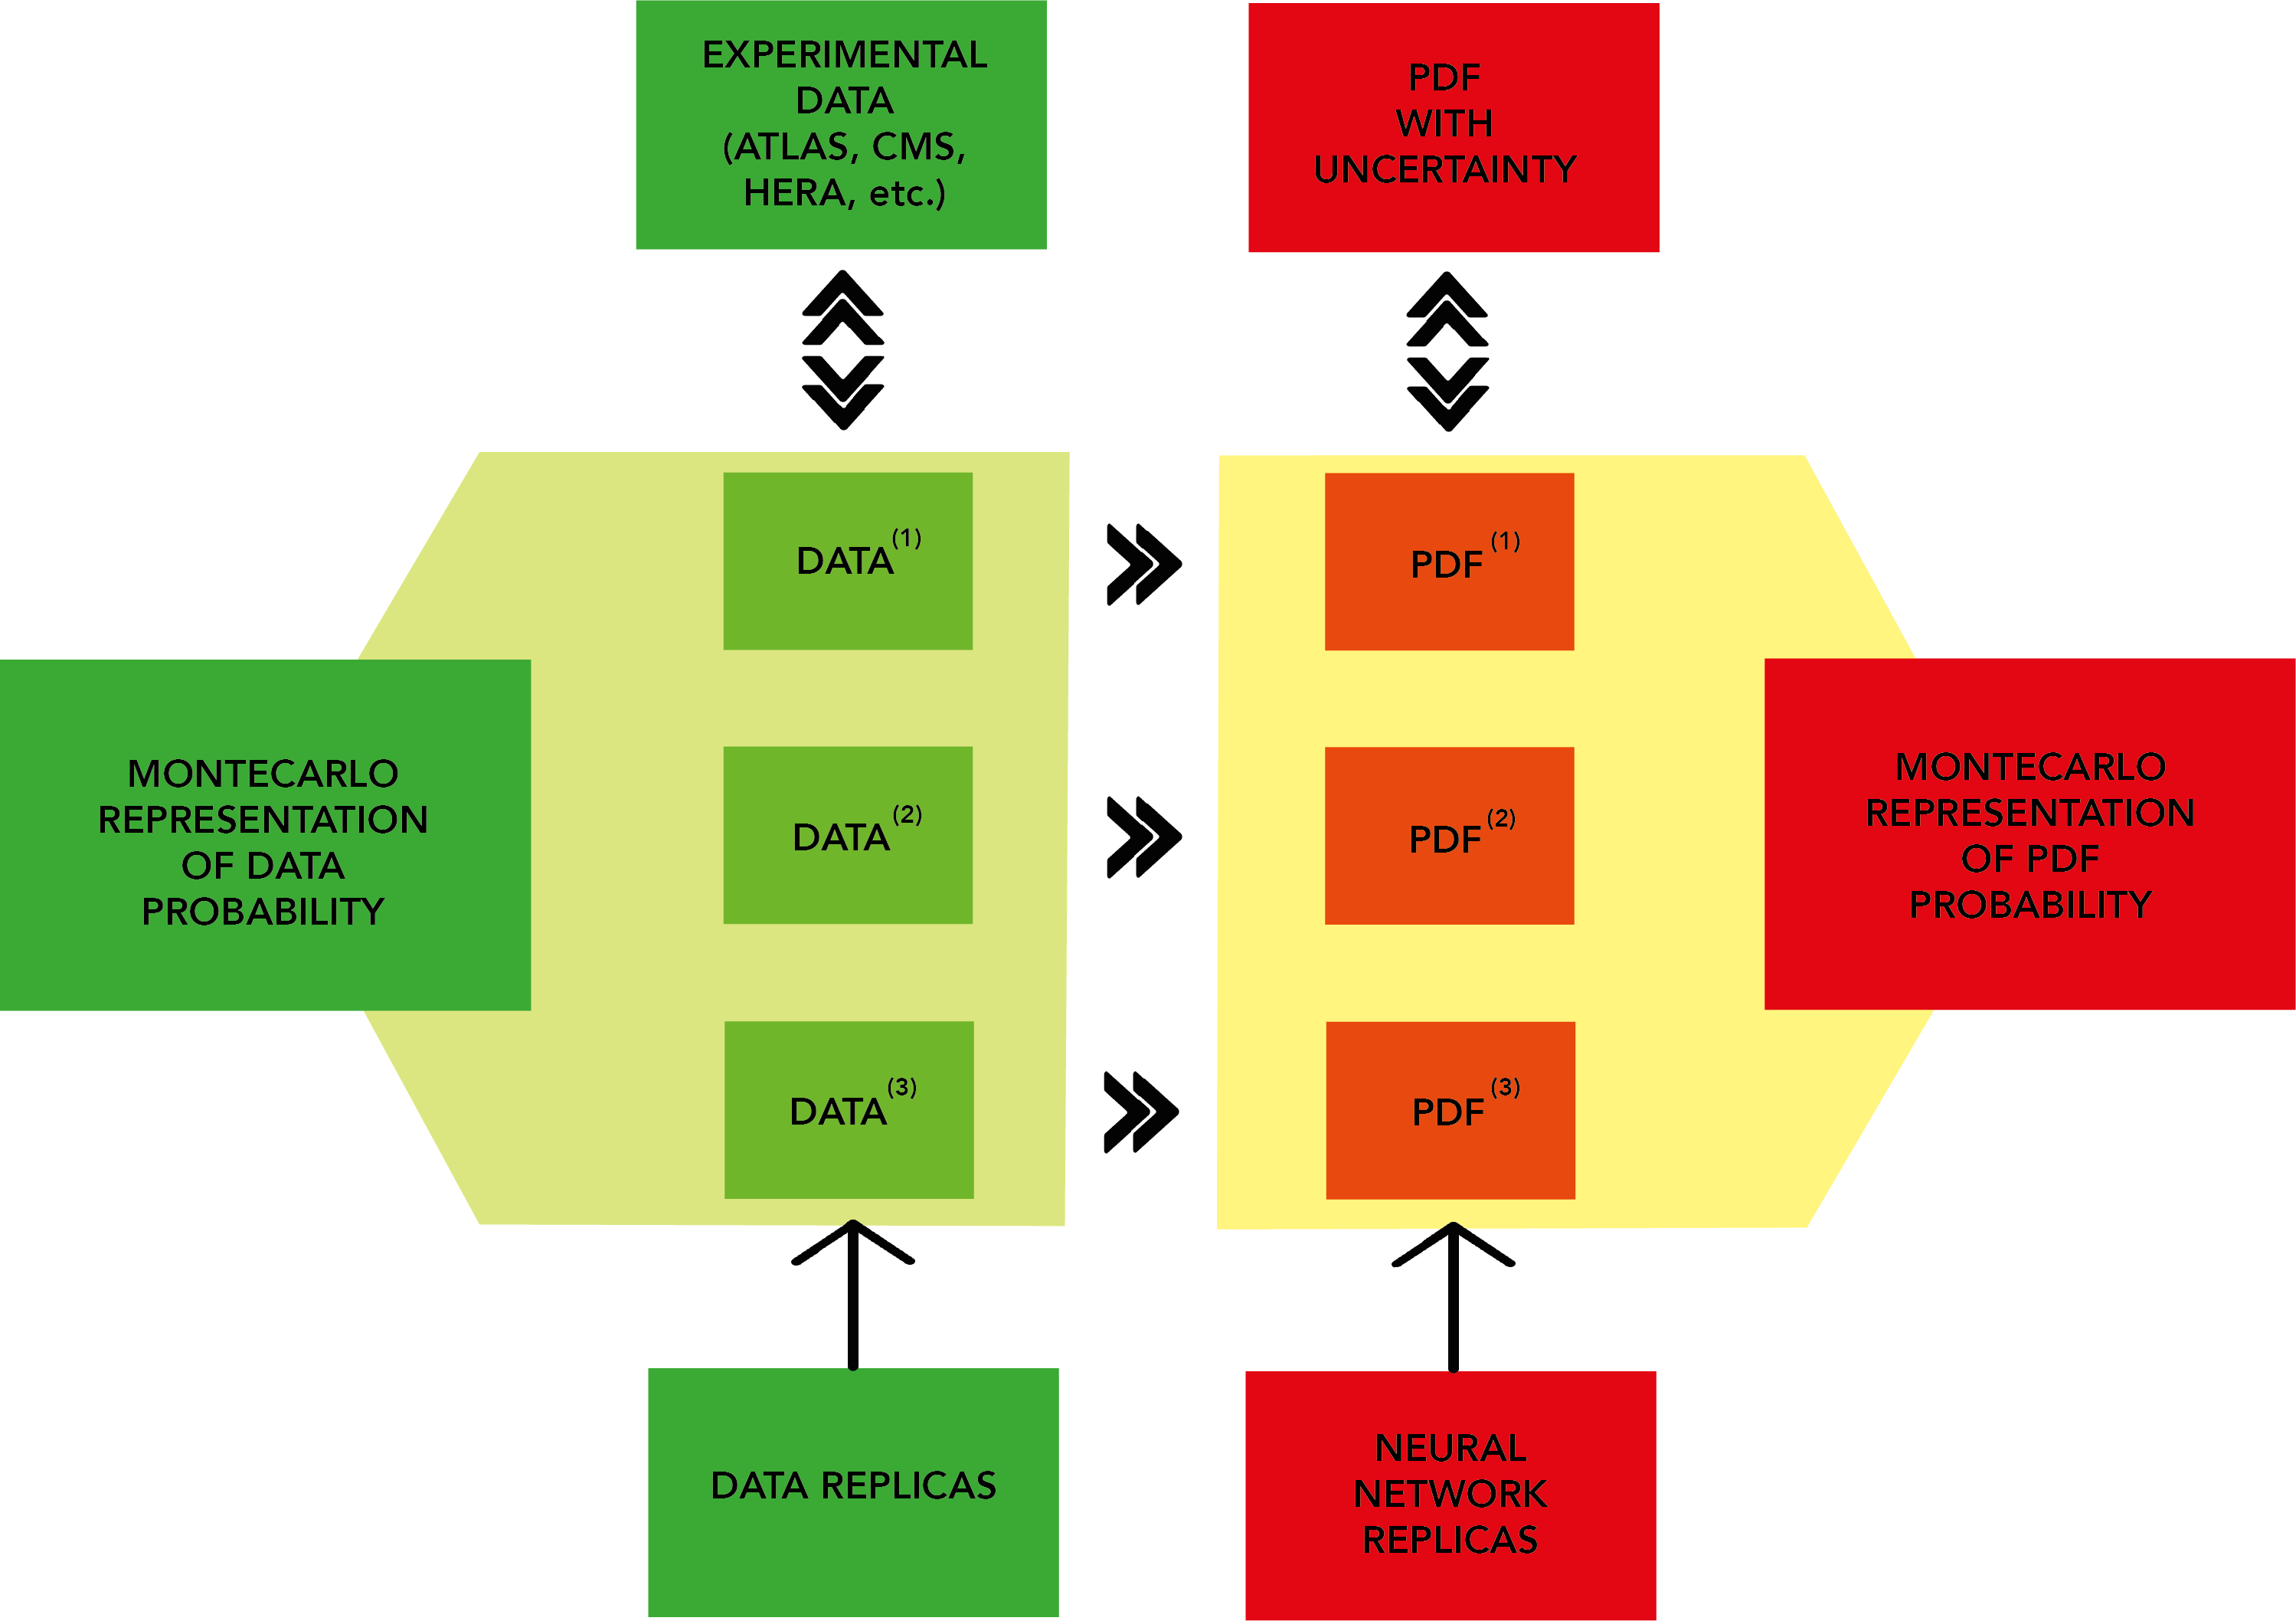
\includegraphics[width=0.5\textwidth]{NNPDF_MC_strategy}
%    \end{center}
%\end{frame}

\begin{frame}[t]{High-precision: gluon}
	\begin{equation*}
	\mathcal{L}_{i j}\left(M_{X}, y, \sqrt{s}\right)
	=\frac{1}{s} \sum_{i, j} f_{i}\left(\frac{M_{X} e^{y}}{\sqrt{s}}, M_{X}\right) f_{j}\left(\frac{M_{X} e^{-y}}{\sqrt{s}}, M_{X}\right)
	\end{equation*}
	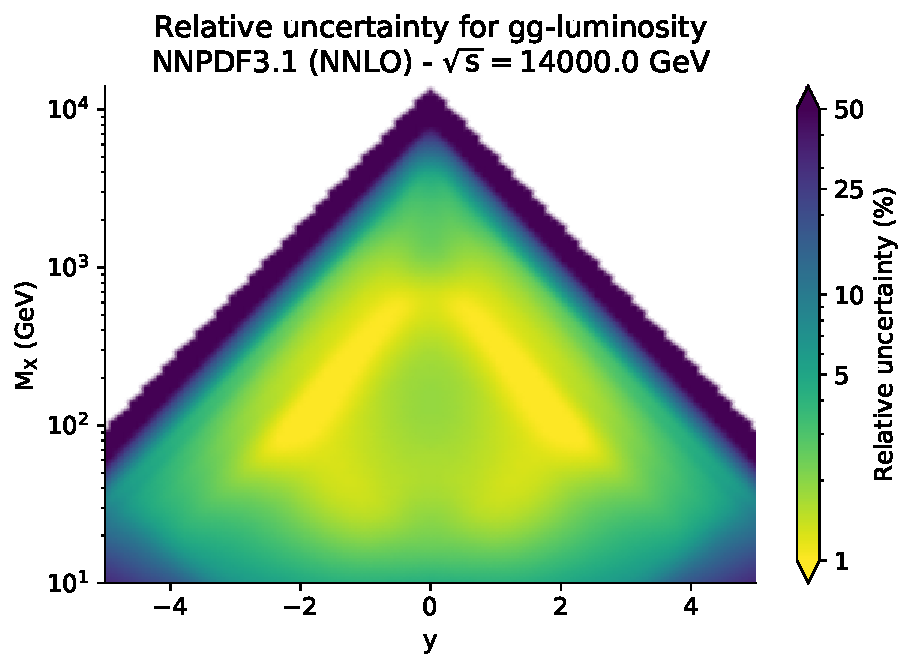
\includegraphics[width=0.45\textwidth]{plot_lumi2d_uncertainty_NNPDF31_gg}
	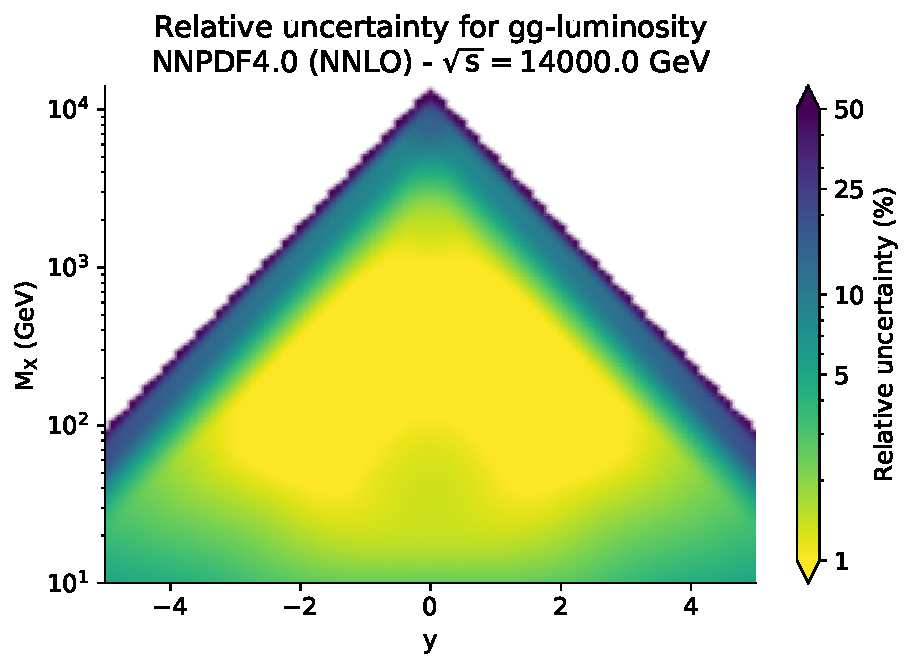
\includegraphics[width=0.45\textwidth]{plot_lumi2d_uncertainty_NNPDF40_gg}
    \begin{center}
	    \textbf{How did we get here?}
	\end{center}
\end{frame}

\begin{frame}[t]{High-precision: singlet }
	\begin{equation*}
	\mathcal{L}_{i j}\left(M_{X}, y, \sqrt{s}\right)
	=\frac{1}{s} \sum_{i, j} f_{i}\left(\frac{M_{X} e^{y}}{\sqrt{s}}, M_{X}\right) f_{j}\left(\frac{M_{X} e^{-y}}{\sqrt{s}}, M_{X}\right)
	\end{equation*}
	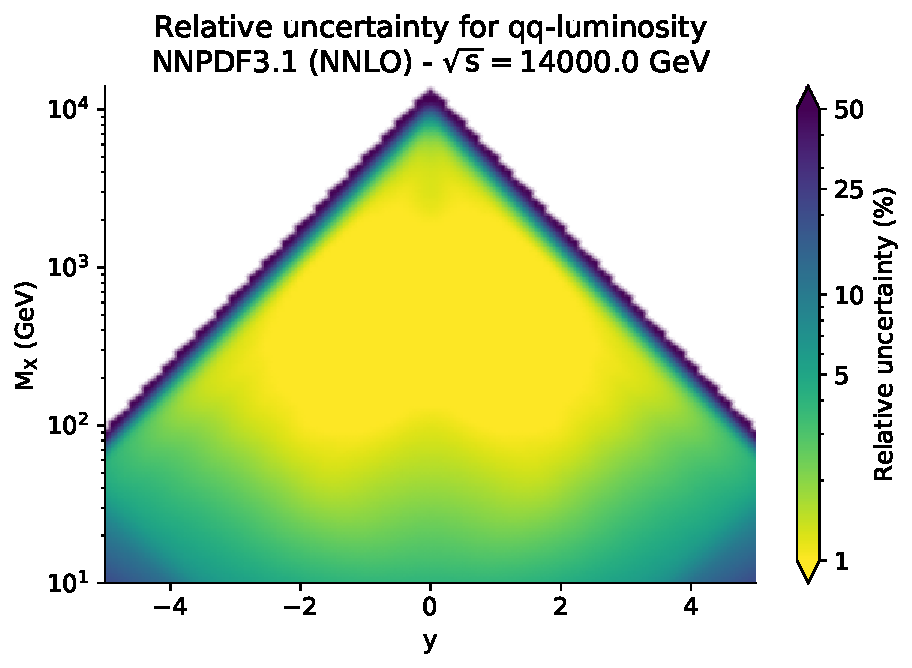
\includegraphics[width=0.45\textwidth]{plot_lumi2d_uncertainty_NNPDF31_qq}
	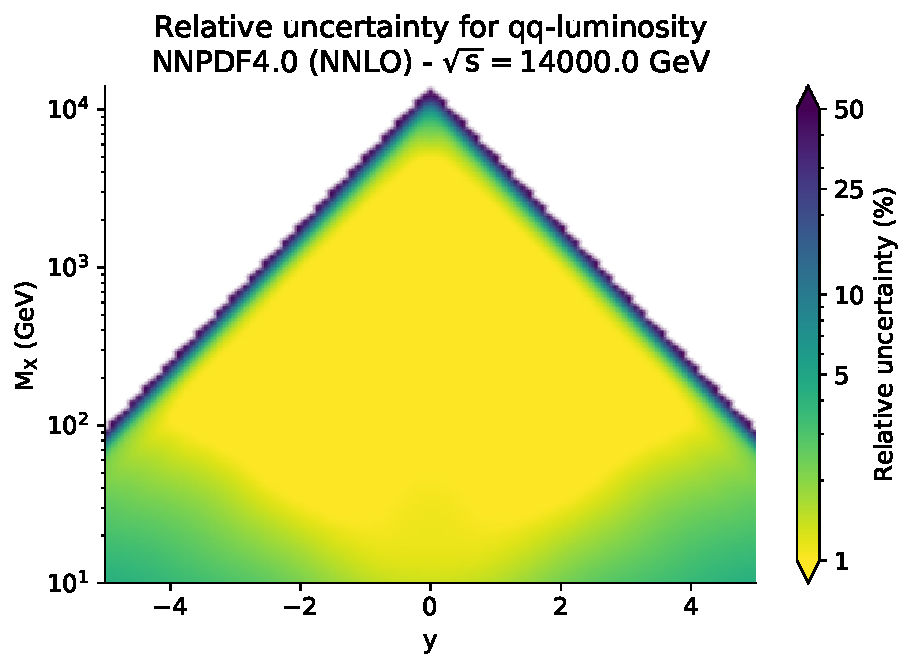
\includegraphics[width=0.45\textwidth]{plot_lumi2d_uncertainty_NNPDF40_qq}\\
	\begin{center}
	    \textbf{How did we get here?}
	\end{center}
\end{frame}


\begin{frame}
 \frametitle{The path to NNPDF4.0}
 \begin{columns}
    \column{0.70\linewidth}
	 \footnotesize
	 \begin{block}{}
	  \centering
	  Progress towards extending {\textcolor{red}{data}}, {\textcolor{blue}{theory}} and {\textcolor{forestgreen}{methodology}}\\
	 \end{block}
	 \scriptsize
	 \renewcommand*{\arraystretch}{1.4}
	 \begin{tabularx}{\textwidth}{lXr}
	  06/2017 & {\bf NNPDF3.1}                                                              
	          & {\tiny{[{\textcolor{salmon}{EPJ\,C77\,(2017)\,663}}]}}\\
	  10/2017 & \textcolor{blue}{NNPDF3.1sx}: {\scriptsize PDFs with small-$x$ resummation}                                                
	          & {\tiny{[{\textcolor{salmon}{EPJ\,C78\,(2018)\,321}}]}}\\
	  12/2017 & \textcolor{blue}{NNPDF3.1luxQED}: {\scriptsize consistent photon PDF \`a la luxQED}                                            
	          & {\tiny{[{\textcolor{salmon}{SciPost\,Phys.\,5\,(2018)\,008}}]}}\\
	  02/2018 & \textcolor{red}{NNPDF3.1+ATLASphoton}: {\scriptsize inclusion of direct photon data}                                       
	          & {\tiny{[{\textcolor{salmon}{EPJ\,C78\,(2018)\,470}}]}}\\
	  12/2018 & \textcolor{forestgreen}{NNPDF3.1alphas}: {\scriptsize $\alpha_s$ from a correlated-replica method}                                     
	          & {\tiny{[{\textcolor{salmon}{EPJ\,C78\,(2018)\,408}}]}}\\
	  12/2018 & \textcolor{forestgreen}{NNPDF3.1nuc}: {\scriptsize heavy ion nuclear uncertainties in a fit}                                        
	          & {\tiny{[{\textcolor{salmon}{EPJ\,C79\,(2019)\,282}}]}}\\
	  05/2019 & \textcolor{forestgreen}{NNPDF3.1th}: {\scriptsize missing higher-order uncertainties in a fit}                                         
	          & {\tiny{[{\textcolor{salmon}{EPJ\,C79\,(2019)\,838; ibid.\,931}}]}}\\
	  07/2019 & \textcolor{forestgreen}{Gradient descent and hyperoptimisation in PDF fits} 
	          & {\tiny{[{\textcolor{salmon}{EPJ\,C79\,(2019)\,676}}]}}\\
	  12/2019 & \textcolor{red}{NNPDF3.1singletop}: {\scriptsize inclusion of single top $t$-channel data}                                          
	          & {\tiny{[{\textcolor{salmon}{JHEP\,05\,(2020)\,067}}]}}\\
	  05/2020 & \textcolor{red}{NNPDF3.1dijets}: {\scriptsize comparative study of single- and di-jets}                                             
	          & {\tiny{[{\textcolor{salmon}{EPJ\,C80\,(2020)\,797}}]}}\\
	  06/2020 & \textcolor{blue}{Positivity of $\overline{\rm MS}$ PDFs}                    
	          & {\tiny{[{\textcolor{salmon}{JHEP\,11\,(2020)\,129}}]}}\\
	  08/2020 & \textcolor{forestgreen}{PineAPPL}: {\scriptsize fast evaluation of EW$\times$QCD corrections}                                           
	          & {\tiny{[{\textcolor{salmon}{JHEP\,12\,(2020)\,108}}]}}\\
	  08/2020 & \textcolor{red}{NNPDF3.1strangeness}: {\scriptsize assessment of strange-sensitive data}                                        
	          & {\tiny{[{\textcolor{salmon}{EPJ\,C80\,(2020)\,1168}}]}}\\
	  11/2020 & \textcolor{forestgreen}{NNPDF3.1deu}: {\scriptsize deuteron uncertainties in a fit}                                        
	          & {\tiny{[{\textcolor{salmon}{EPJ\,C81\,(2021)\,37}}]}}\\
	  03/2021 & \textcolor{forestgreen}{Future tests}                                       
	          & {\tiny{[{\textcolor{salmon}{arXiv:2103.08606}}]}}\\
	  2021    & {\bf NNPDF4.0}                                                              
	          & {\tiny{[{\textcolor{salmon}{to appear}}]}}\\
	 \end{tabularx}
    \end{columns}
\end{frame}


\section*{Dataset}



\begin{frame}{Experimental data in NNPDF4.0}
	\begin{columns}
	    \column{0.48\linewidth}
	        {\footnotesize
	        \begin{itemize}
	            \item $\mathcal{O}(35)$ datasets investigated
	            \item $\mathcal{O}(400)$ more data points in NNPDF4.0 \\ than in NNPDF3.1
	            \item New data is mostly from the LHC RUN II
	        \end{itemize}
	        }
	        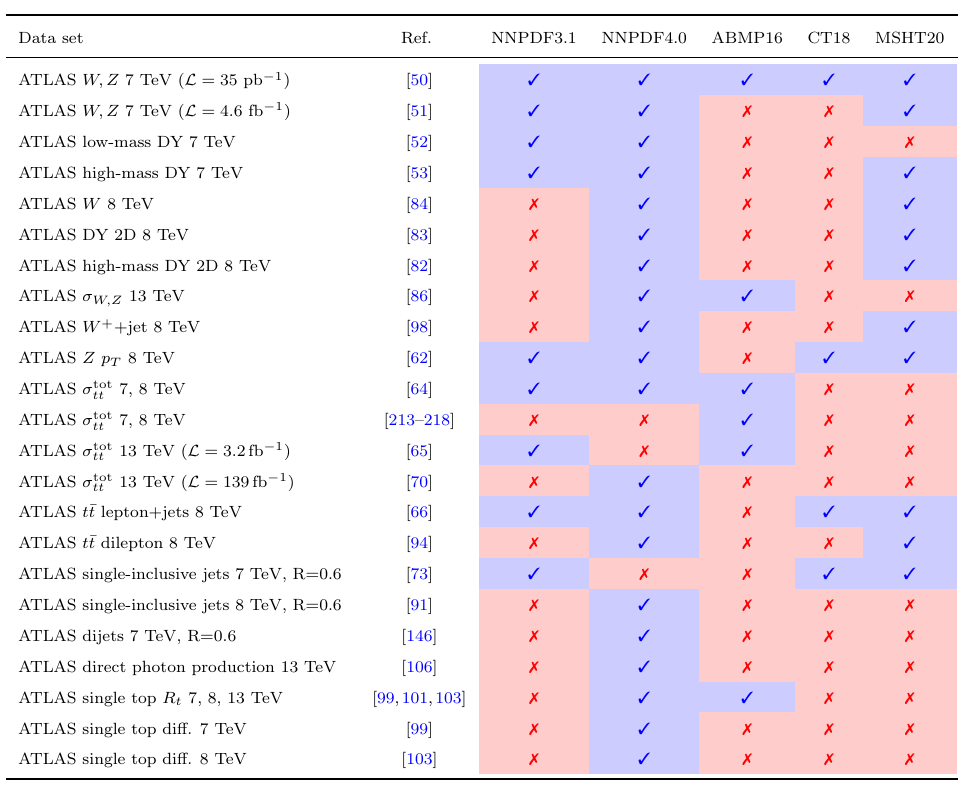
\includegraphics[width=0.9\textwidth]{atlas_data_table}
	
	    \column{0.48\linewidth}
	        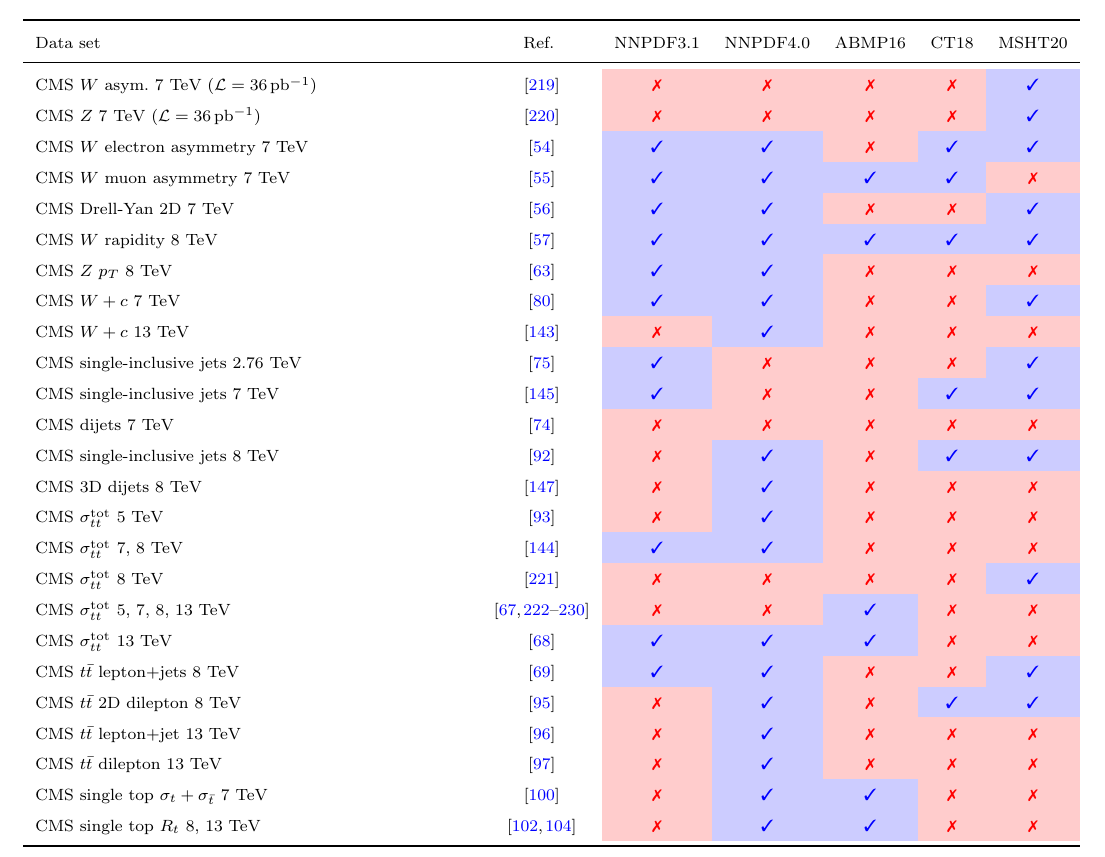
\includegraphics[width=0.9\textwidth]{cms_data_table} \\
	        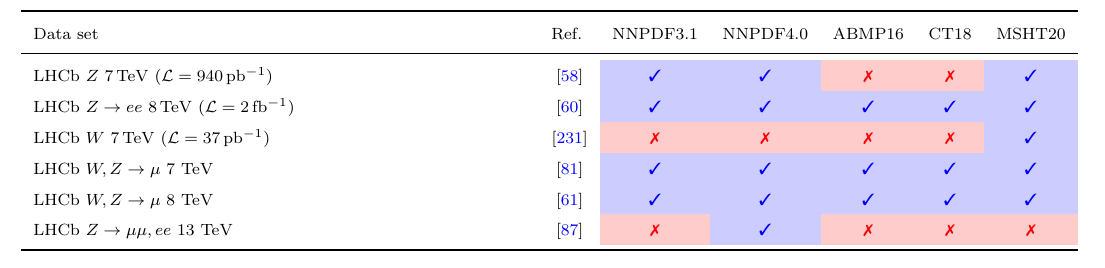
\includegraphics[width=0.9\textwidth]{lhcb_data_table}
	\end{columns}
\end{frame}


\begin{frame}{Experimental data in NNPDF4.0}
    \begin{columns}
        \column{0.7\linewidth}
            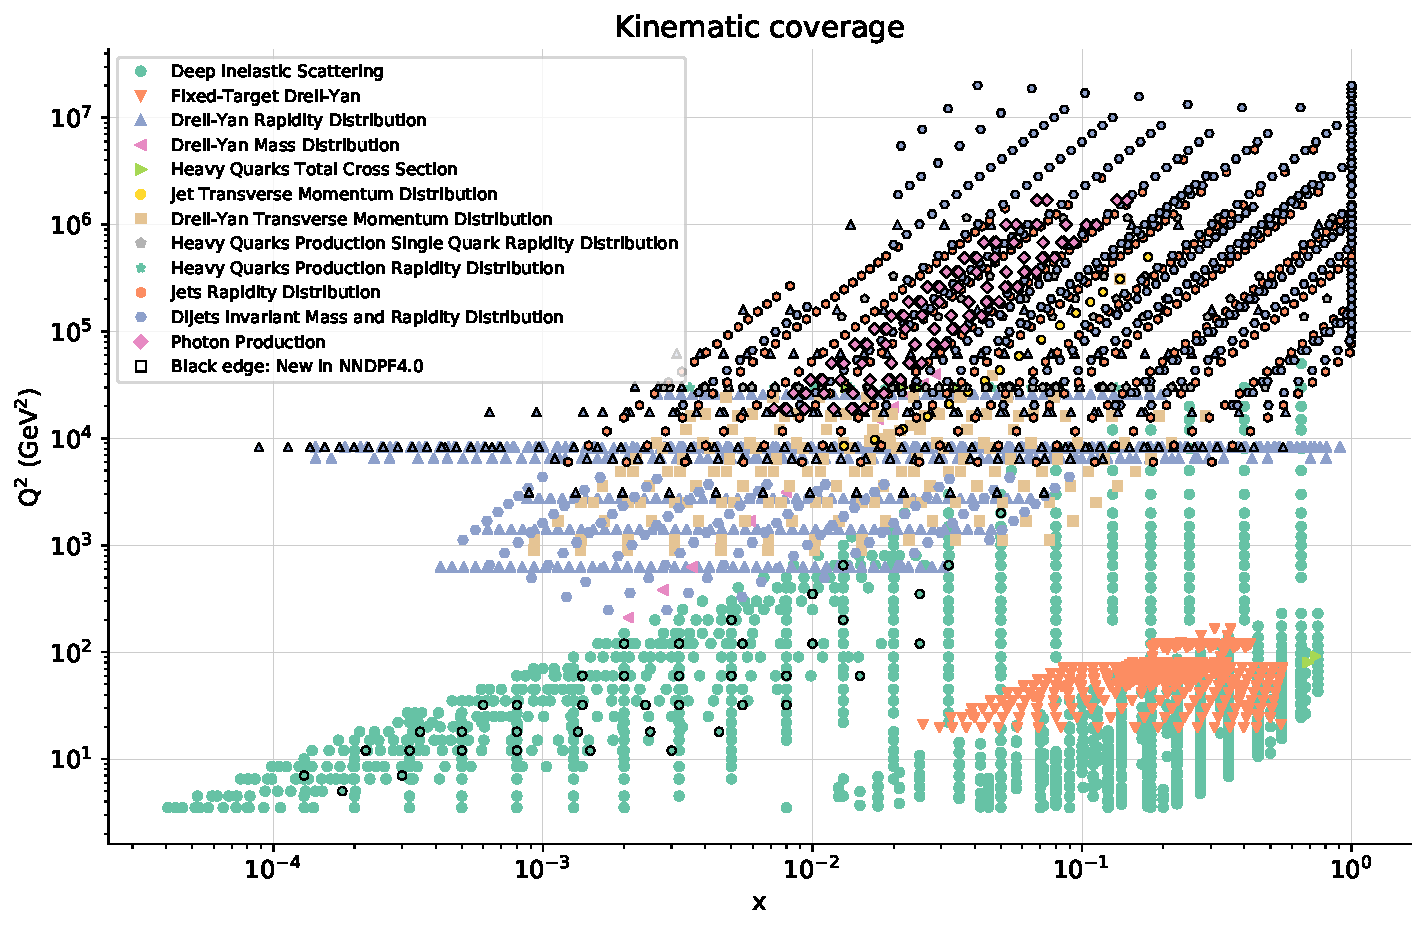
\includegraphics[width=1.0\textwidth]{Markers0_plot_xq2}
        \column{0.25\linewidth}
            New processes:
            \begin{itemize}
                \item direct photon
                \item single top
                \item dijets
                \item W+jet
                \item DIS jet
            \end{itemize}
    \begin{block}{\footnotesize Theoretical improvement}
    {\footnotesize
    Nuclear uncertainties are included
    }
    \end{block}
    \end{columns}
\end{frame}




\section*{Methodology}




%\begin{frame}[t]
%    \frametitle{Improved fitting methodology}
%    \footnotesize
%    \begin{columns}[t]
%        \column{0.5\linewidth}
%            \mycolutitle{NNPDF 3.1 code}
%            \begin{list}{\color{darkred} $\rightarrow$}{}  
%                \item {\bf Fit parameters manually chosen }
%                \item {\bf Fitting times of up to various days}
%                \item { Genetic Algorithm optimizer}
%                \item One network per flavour
%                \item Physical constraints imposed independently of optimization
%                \item Preprocessing fixed per each of the replicas
%                \item C++ monolithic codebase
%                \item In-house Machine Learning optimization framework
%            \end{list}
%        \column{0.5\linewidth}
%            \mycolutitle{NNPDF 4.0 code}
%            \begin{list}{\color{darkgreen} $\rightarrow$}{}
%                \item {\bf Fit parameters chosen automatically (hyperparameter scan)}
%                \item {\bf Results available in less than an hour}
%                \item {Gradient Descent optimization}
%                \item One network for all flavours
%                \item Physical constraints integrated in the optimization
%                \item Preprocessing can be fitted within replicas
%                \item Python object oriented codebase
%                \item Freedom to use external libraries (default: TensorFlow)
%            \end{list}
%    \end{columns}
%\end{frame}


\begin{frame}[t]{Improved fitting methodology}
    \begin{columns}[T]
        \begin{column}{0.48\textwidth}
            \begin{itemize}
                \item \textbf{Stochastic Gradient Descent} for NN training using TensorFlow
%                \item Factor $\sim$ 25 \textbf{reduction in fit time}
                \item Automated \textbf{hyperparameter optimization}
                \item Accuracy of the \textbf{uncertainty is validated} using 
                {\bf closure tests} (data region), {\bf future tests} (extrapolation region), and {\bf parametrization basis independence}
            \end{itemize}
        \vspace*{1em}
        Physical constraints:
        \begin{itemize}
            \item PDF positivity {\footnotesize{{\textcolor{blue}{[JHEP\,11\,(2020)\,129]}}}}
            \item Integrability of nonsinglet distributions (Gottfried sum rules)
        \end{itemize}
        \end{column}
        \begin{column}{0.48\textwidth}
            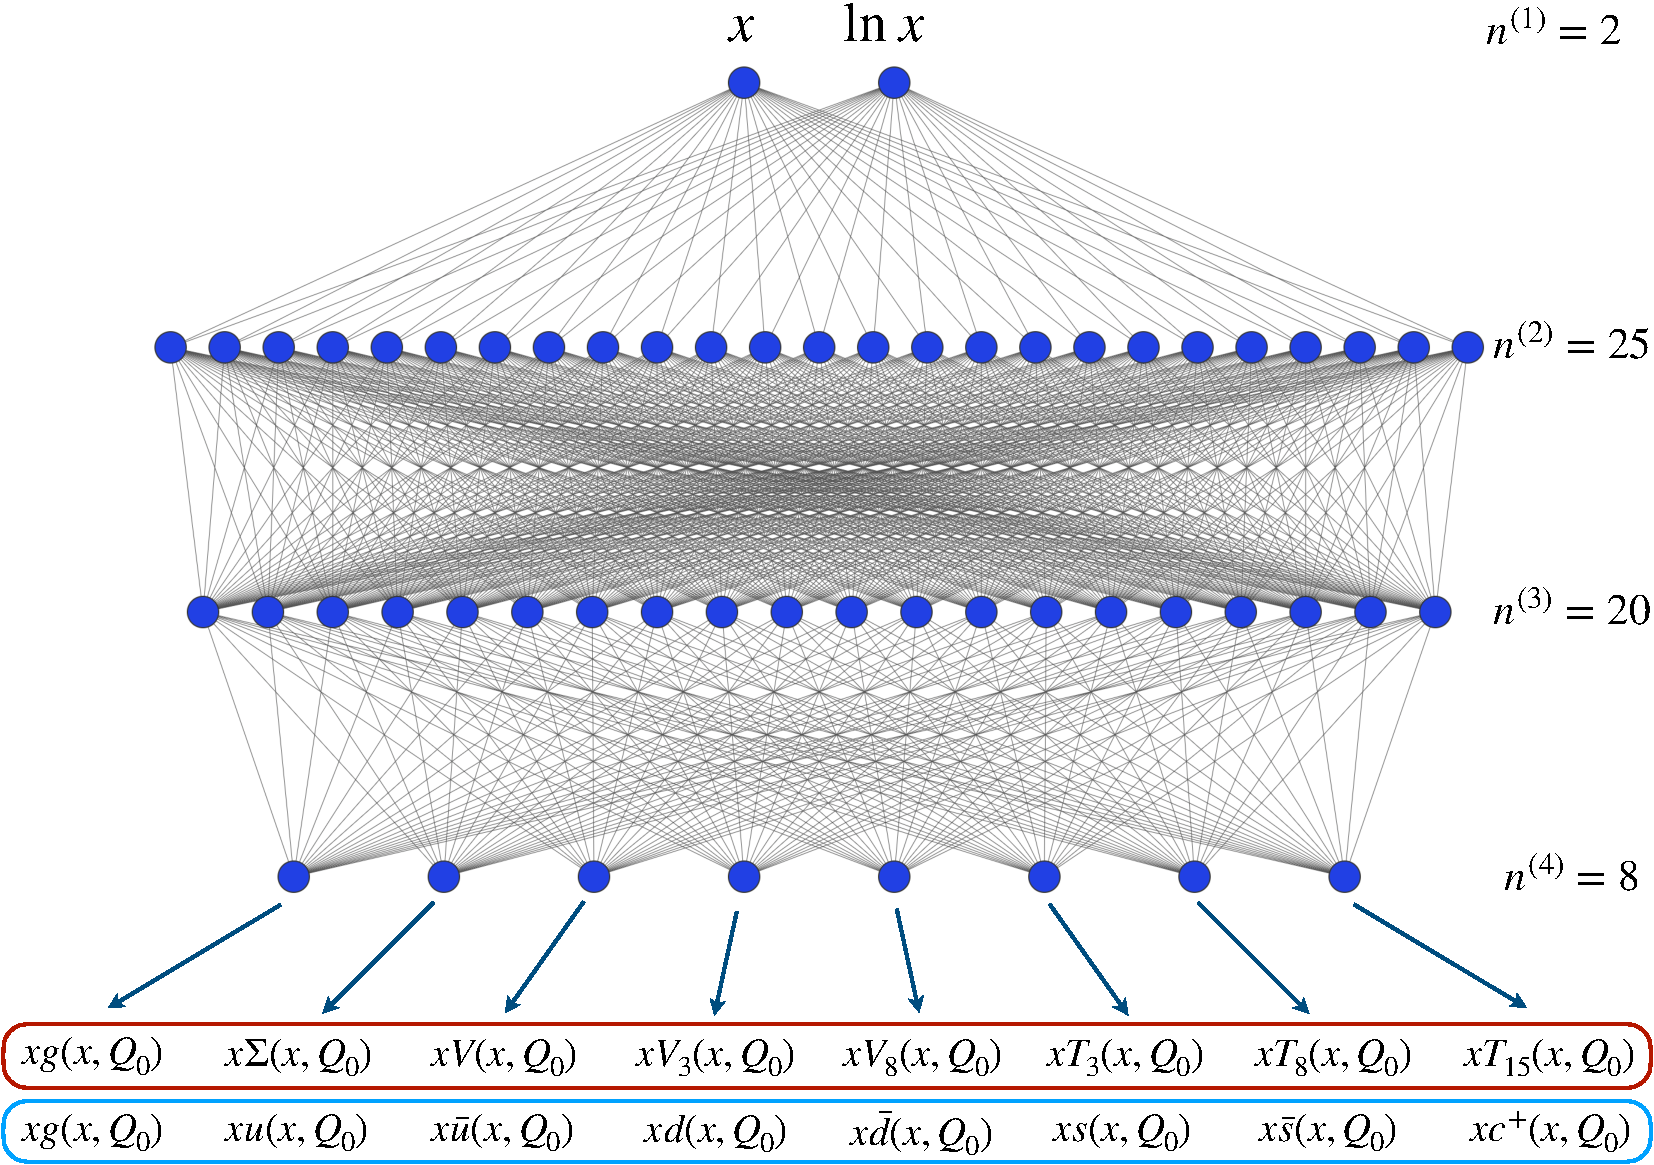
\includegraphics[width=1.0\textwidth]{NNarch}
            \begin{equation*}
                f_{i}\left(x, Q_{0}\right)=x^{-\alpha_{i}}(1-x)^{\beta_{i}} \mathrm{NN}_{i}(x)
            \end{equation*}
        \end{column}
    \end{columns}
\end{frame}


\begin{frame}{Parametrization basis independence}
    \begin{columns}
        \begin{column}[T]{0.48\textwidth}
        \vspace*{0pt}%
	        \begin{center}
	            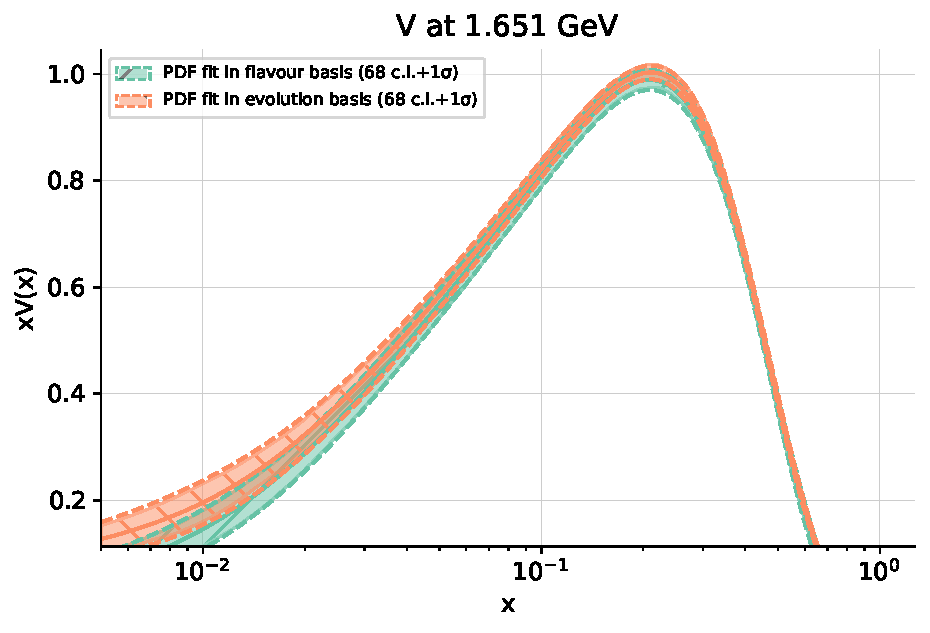
\includegraphics[width=0.8\textwidth]{flavour_evolution_V} \\
	        \end{center}
%            Evolution Basis:
%            {\footnotesize
%            \begin{equation*}
%				\begin{array}{l}
%				    q_{k}\left(x, Q_{0}\right) \propto x^{-\alpha_{k}}(1-x)^{\beta_{k}} N N(x) \\
%				    q_{k}=\left\{V, V_{3}, V_{8}, T_{3}, T_{8}, T_{15}, \Sigma, g\right\}
%				\end{array}
%            \end{equation*}

%            }
%            Evolution Basis:
%            {\footnotesize
%			\begin{equation*}
%				\begin{array}{l}
%					q_{k}\left(x, Q_{0}\right) \propto(1-x)^{\beta_k} N N(x) \\
%					q_{k}=\{u, \bar{u}, d, \bar{d}, s, \bar{s}, c, g\}
%				\end{array}
%			\end{equation*}
%        }
        \end{column}
        \begin{column}[t]{0.48\textwidth}
        \vspace{0pt}%
	        \begin{center}
	            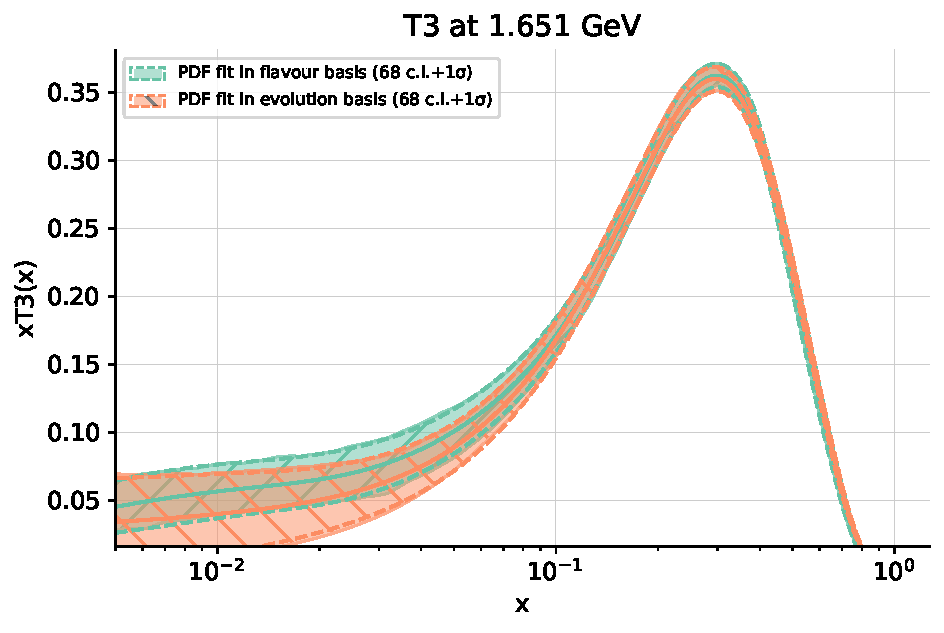
\includegraphics[width=0.8\textwidth]{flavour_evolution_T3} \\
	        \end{center}
%	        Physical constraint:
%	        \begin{itemize}
%	            \item PDF positivity
%	            \item Integrability of nonsinglet distributions
%	        \end{itemize}
        \end{column}
    \end{columns}
    \begin{columns}
        \column{0.4\linewidth}
		    Evolution Basis:
		    {\footnotesize
		    \begin{fleqn}
		    \begin{align*}
		       \qquad x V\left(x, Q_{0}\right) &\propto \mathrm{NN}_{V}(x)\\
		        x T_{3}\left(x, Q_{0}\right) &\propto \mathrm{NN}_{T_{3}}(x)
		    \end{align*}
		    \end{fleqn}
		    }
        \column{0.55\linewidth}
            \begin{block}{}
                \textbf{Different strategies} to parametrize the quark PDF flavour combinations lead to \textbf{identical results}
            \end{block}
    \end{columns}
    \vspace*{-0.5em}
    Flavour Basis:
    {\footnotesize
    \begin{fleqn}
    \begin{align*}
        \qquad x V\left(x, Q_{0}\right) &\propto\left(\mathrm{NN}_{u}(x)-\mathrm{NN}_{\bar{u}}(x)+\mathrm{NN}_{d}(x)-\mathrm{NN}_{\bar{d}}(x)+\mathrm{NN}_{s}(x)-\mathrm{NN}_{\bar{s}}(x)\right) \\
        x T_{3}\left(x, Q_{0}\right) &\propto\left(\mathrm{NN}_{u}(x)+\mathrm{NN}_{\bar{u}}(x)-\mathrm{NN}_{d}(x)-\mathrm{NN}_{\bar{d}}(x)\right)
    \end{align*}
    \end{fleqn}
    }
\end{frame}



\begin{frame}[t]{Learning the methodology}
	NNPDF aims to minimize sources of bias in the PDF:
	\begin{itemize}
	    \item Functional form $\rightarrow$ Neural Network
	    \item Model parameters $\rightarrow$ ?
	\end{itemize}
\end{frame}


\begin{frame}[t]{Learning the methodology}
	NNPDF aims to minimize sources of bias in the PDF:
	\begin{itemize}
	    \item Functional form $\rightarrow$ Neural Network
	    \item Model parameters $\rightarrow$ \textbf{Hyperoptimization}
	\end{itemize}
	\begin{center}
	    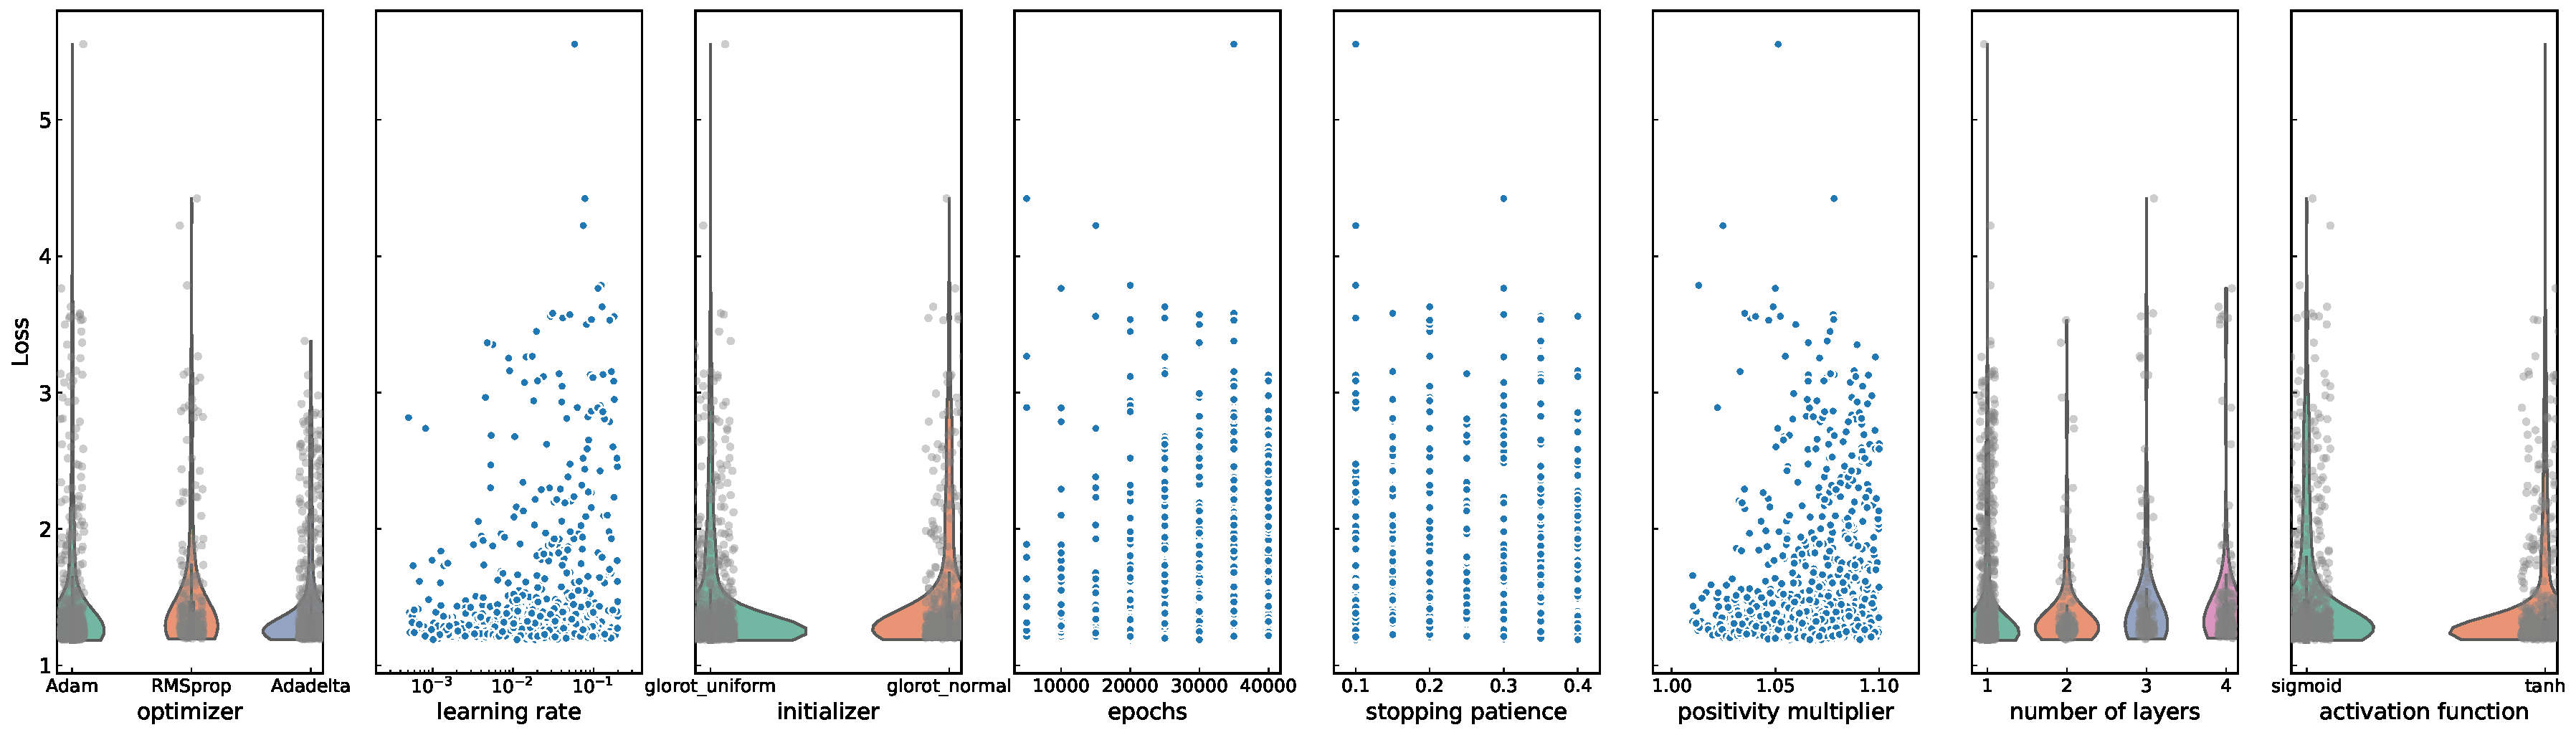
\includegraphics[width=0.9\textwidth]{hyperopt_scan}
	\end{center}
    Scan over thousands of hyperparameter combinations and select the best one \\
    {\bf k-fold cross-validation}: used to define the reward function based on {\bf test dataset}
\end{frame}


%\begin{frame}[t]{Hyperoptimization: the reward function}
%    \begin{columns}[T]
%        \begin{column}{0.48\textwidth}
%            \vspace{\topsep}
%            Choosing as the hyperoptimization target the $\chi^2$ of fitted data results in overfitting.
%        \end{column}
%        \begin{column}{0.48\textwidth}
%            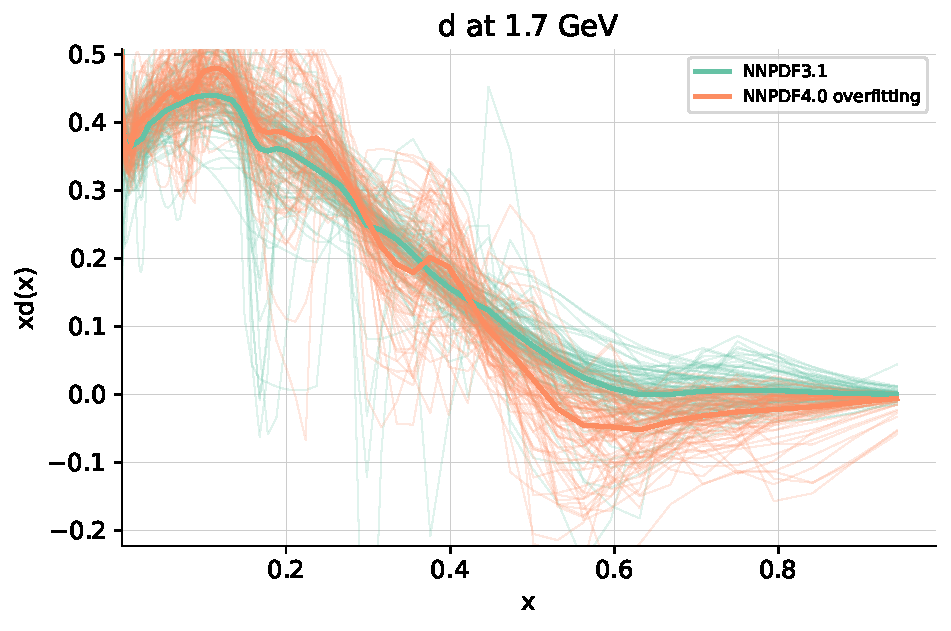
\includegraphics[width=0.9\textwidth]{overfit_nnpdf31}
%        \end{column}
%    \end{columns}
%\end{frame}



%\begin{frame}[t]{Hyperoptimization: the reward function}
%    \begin{columns}[T]
%        \begin{column}{0.48\textwidth}
%            \vspace{\topsep}
%            Choosing as the hyperoptimization target the $\chi^2$ of fitted data results in overfitting.\\
%			\vspace*{2em}			
%			We solve this using \textbf{k-fold cross-validation}:
%			\begin{enumerate}
%			    \item Divide the data into $k$ {representative subsets}
%			    \item Fit $k-1$ sets and use $k$-th as test set
%			    \begin{itemize}
%			        \item[$\Rightarrow$] $k$ values of $\chi^2_\mathrm{test}$
%			    \end{itemize}
%			    \item Optimize the average $\chi^2_\mathrm{test}$ of the $k$ test sets
%			\end{enumerate}
%			\vspace*{0.5em}
%			$\Rightarrow$ The hyperoptimization target is not based on data that entered the fit. 
%        \end{column}
%        \begin{column}{0.48\textwidth}
%            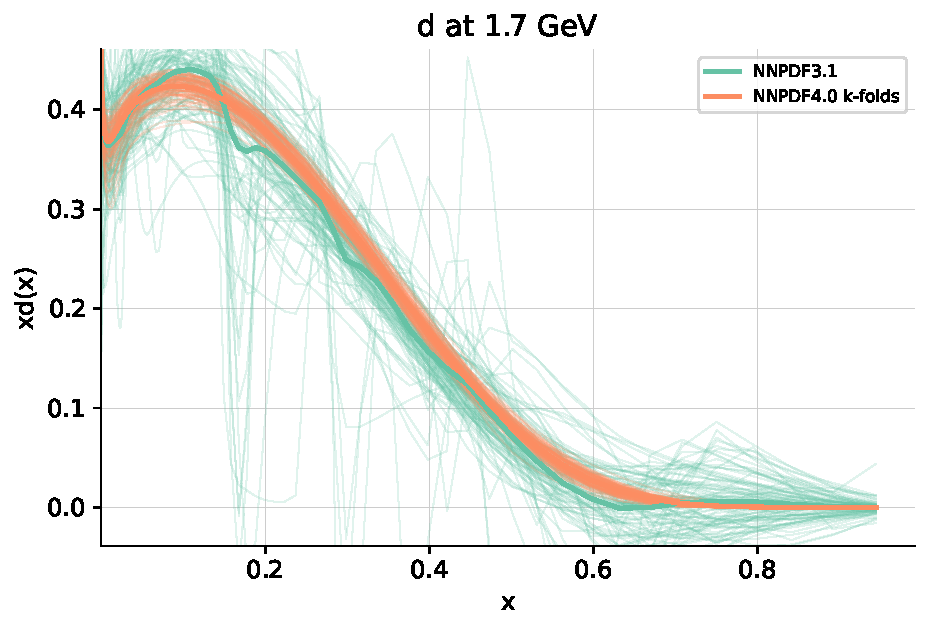
\includegraphics[width=0.9\textwidth]{best_model_vs_nnpdf31}
%            \begin{itemize}
%                \item No overfitting\\
%			    \vspace*{0.2em}
%			    \item Compared to NNPDF3.1:
%			    \begin{itemize}
%			        \item Increased stability
%			        \item Reduced uncertainties 
%			    \end{itemize}
%			\end{itemize}
%        \end{column}
%    \end{columns}
%\end{frame}





\section*{PDFs and Phenomenology}




%\begin{frame}
% \frametitle{Impact of the new data and fitting methodology}
% \footnotesize
% \centering
% \begin{columns}[c]
%  \begin{column}{0.5\textwidth}
%   \begin{overlayarea}{\columnwidth}{4cm}
%    \only<1>
%    {
%     \centering
%     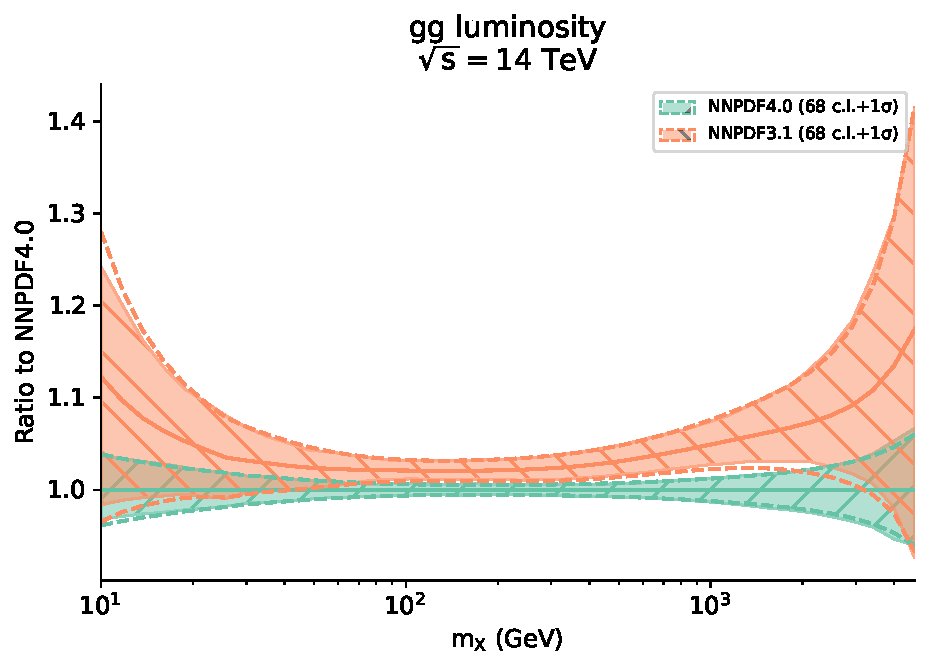
\includegraphics[width=0.65\columnwidth]{lumi1d_gg_NNPDF31_NNPDF40}\\    
%    }
%    \only<2>
%    {
%     \centering
%     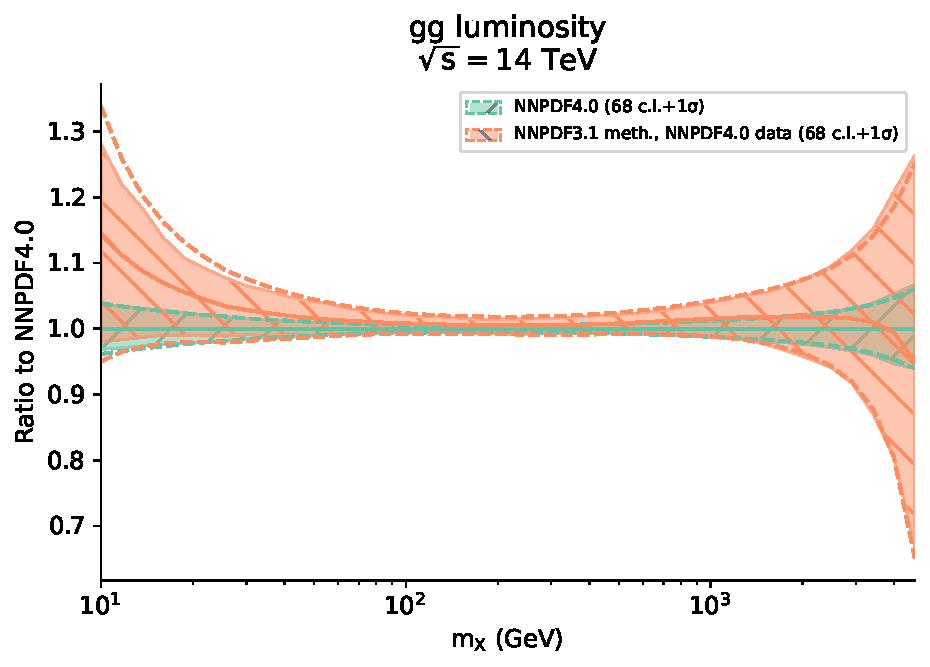
\includegraphics[width=0.65\columnwidth]{lumi1d_gg_NNPDF31meth_NNPDF40}\\    
%    }
%   \end{overlayarea}
%  \end{column}
%  \begin{column}{0.5\textwidth}
%   \begin{overlayarea}{\columnwidth}{4cm}
%    \vspace*{-0.6cm}    
%    \only<1>
%    {
%     \centering
%     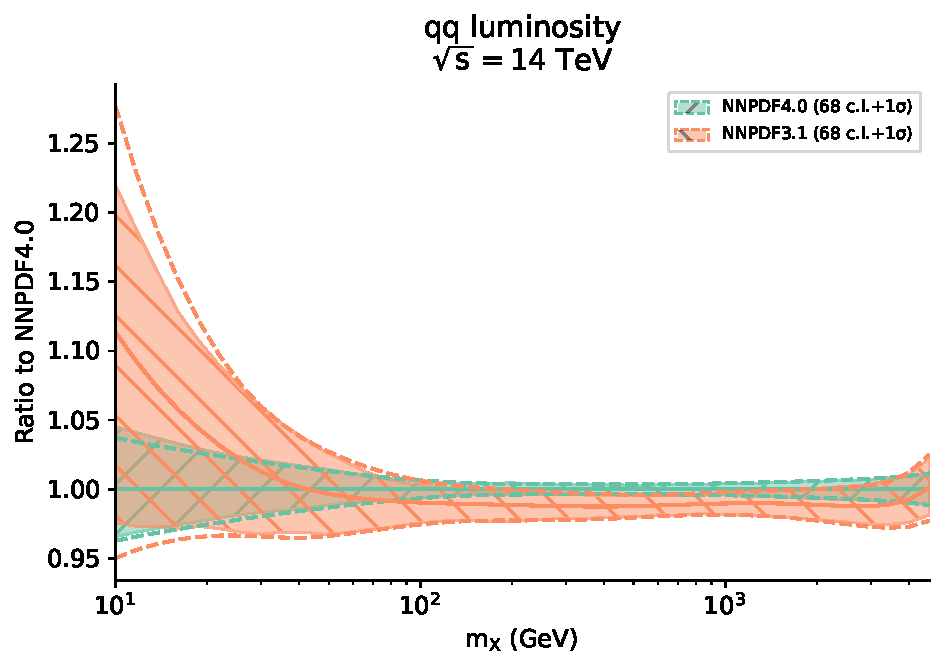
\includegraphics[width=0.65\columnwidth]{lumi1d_qq_NNPDF31_NNPDF40}\\    
%    }
%    \only<2>
%    {
%     \centering
%     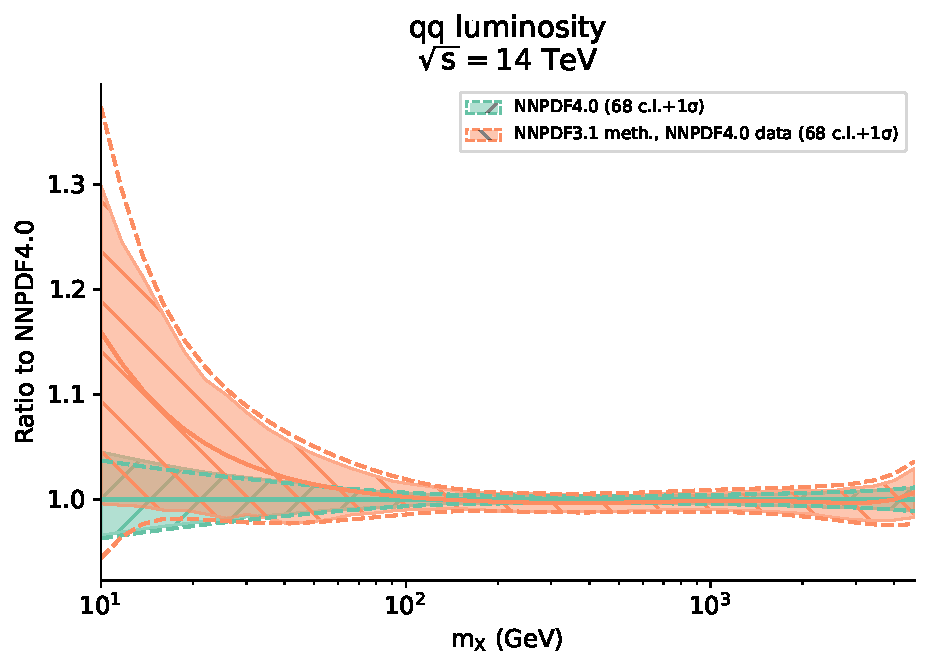
\includegraphics[width=0.65\columnwidth]{lumi1d_qq_NNPDF31meth_NNPDF40}\\    
%    }
%   \end{overlayarea}   
%  \end{column} 
% \end{columns}
% \begin{columns}[c]
%  \begin{column}{0.5\textwidth}
%   \begin{overlayarea}{\columnwidth}{4cm}
%    \vspace*{-0.55cm}
%    \only<1>
%    {
%     \centering
%     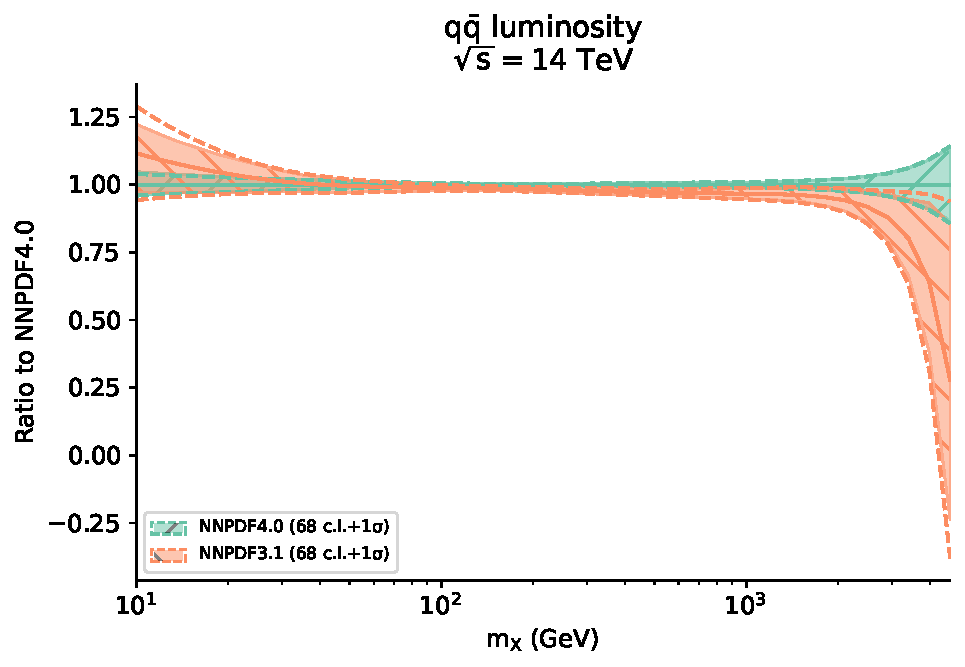
\includegraphics[width=0.65\columnwidth]{lumi1d_qqb_NNPDF31_NNPDF40}\\
%    }
%    \only<2>
%    {
%     \centering
%     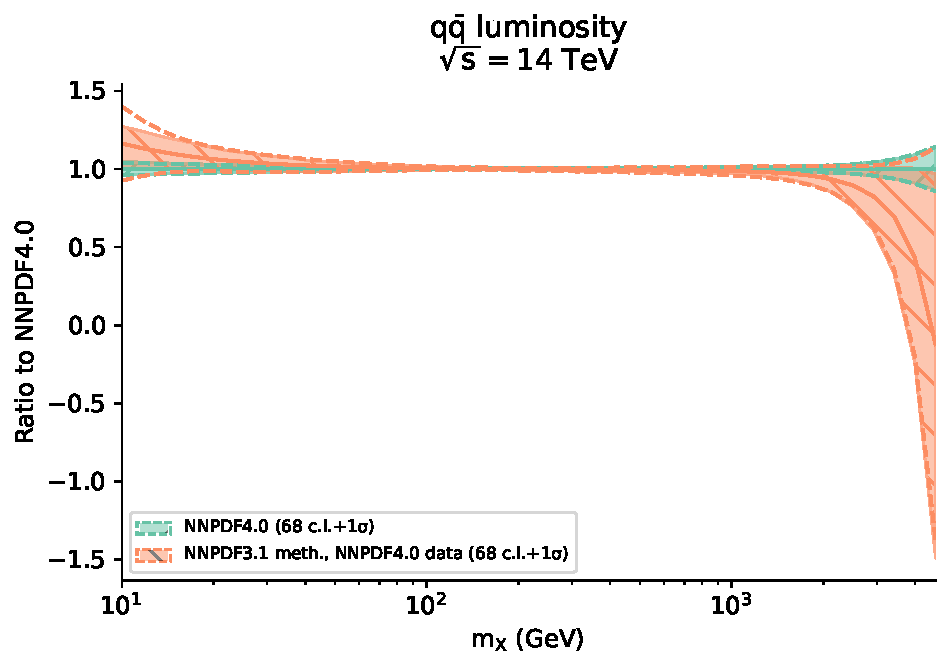
\includegraphics[width=0.65\columnwidth]{lumi1d_qqb_NNPDF31meth_NNPDF40}\\    
%    }
%   \end{overlayarea}   
%  \end{column}
%  \begin{column}{0.5\textwidth}
%   \begin{overlayarea}{\columnwidth}{4cm}
%    \vspace*{-0.8cm}    
%    \only<1>
%    {
%     \centering
%     \tiny
%     \renewcommand*{\arraystretch}{1.35}
%     \begin{tabular}{lcc}
%      \toprule
%       \backslashbox{data set ($N_{\rm dat}$)}{methodology} & NNPDF3.1         & NNPDF4.0        \\
%       \midrule
%       NNPDF3.1 (4093)                                     & \alert{\bf 1.19} &            1.11  \\
%       NNPDF4.0 (4618)                                     &      1.25        & \alert{\bf 1.16} \\
%      \bottomrule
%     \end{tabular}\\
%     \vspace{0.3cm}
%%     \scriptsize
%%     \underline{Consistency} between PDF sets\\
%%     \vspace{0.2cm}
%%     NNPDF4.0 \underline{more precise}\\
%%     (combination of data set and methodology)\\
%%     \vspace{0.2cm}
%%     NNPDF4.0 \underline{more accurate}\\
%%     (superiority of the NNPDF4.0 methodology)\\
%    }
%    \only<2>
%    {
%      \centering
%     \tiny
%     \renewcommand*{\arraystretch}{1.35}
%     \begin{tabular}{lcc}
%      \toprule
%       \backslashbox{data set ($N_{\rm dat}$)}{methodology} & NNPDF3.1         & NNPDF4.0        \\
%       \midrule
%       NNPDF3.1 (4093)                                      &            1.19  &            1.11  \\
%       NNPDF4.0 (4618)                                      & \alert{\bf 1.25} & \alert{\bf 1.16} \\
%      \bottomrule
%     \end{tabular}\\
%     \vspace{0.3cm}
%%     \scriptsize
%%     \underline{Consistency} between PDF sets\\
%%     \vspace{0.2cm}
%%     NNPDF4.0 \underline{more precise}\\
%%     (combination of data set and methodology)\\
%%     \vspace{0.2cm}
%%     NNPDF4.0 \underline{more accurate}\\
%%     (superiority of the NNPDF4.0 methodology)\\  
%      {Moderate reduction of PDF ucertainties \\
%      shifts in central values at the one-sigma level}
%    }
%   \end{overlayarea}   
%  \end{column}   
% \end{columns}
%\end{frame}


\begin{frame}[t]{Impact of the new data}
%    \begin{center}
%        Consistency between data sets \\
%    \end{center}
	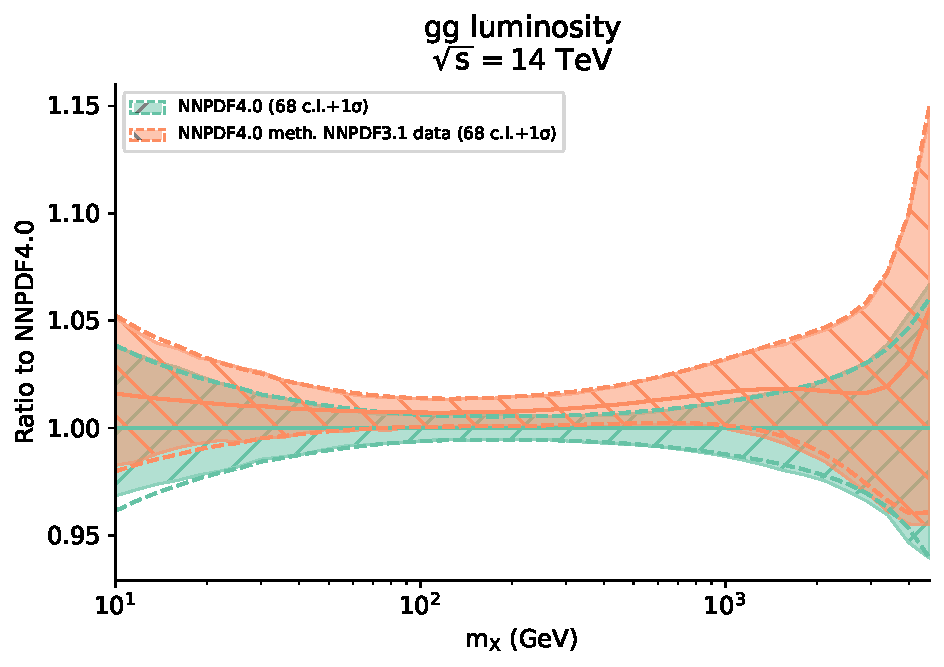
\includegraphics[width=0.45\textwidth]{lumi1d_gg_NNPDF40meth_NNPDF31data}
	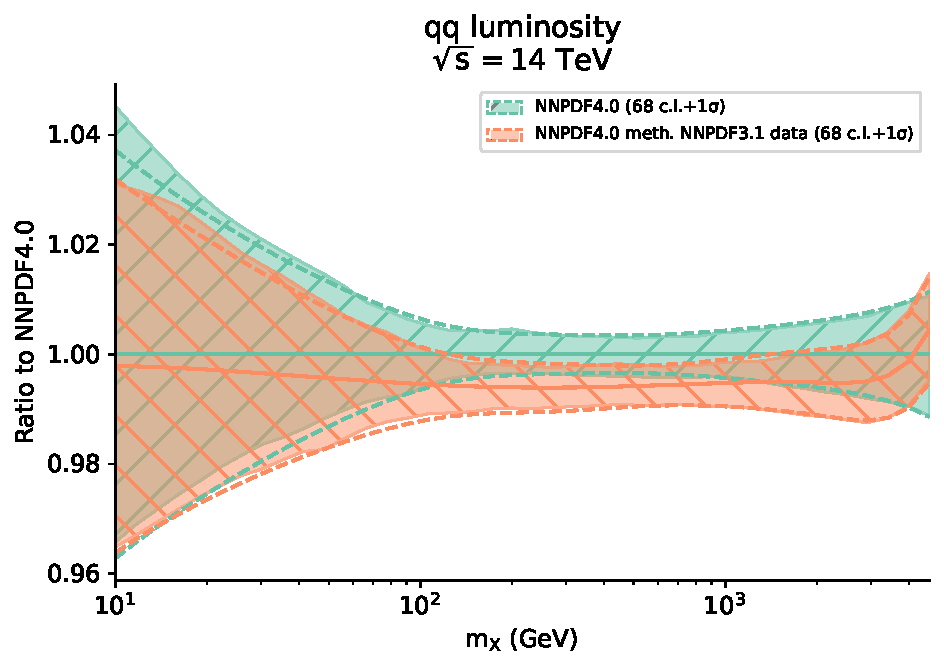
\includegraphics[width=0.45\textwidth]{lumi1d_qq_NNPDF40meth_NNPDF31data}
	Individual datasets have a limited impact, but collectively they result in:
	\begin{itemize}
	    \item Moderate reduction of PDF uncertainties
	    \item Shifts in central value at the one-sigma level
	\end{itemize}
\end{frame}


\begin{frame}[t]{Impact of the new fitting methodology}
%    \begin{center}
%        Consistency between methodologies \\
%    \end{center}
	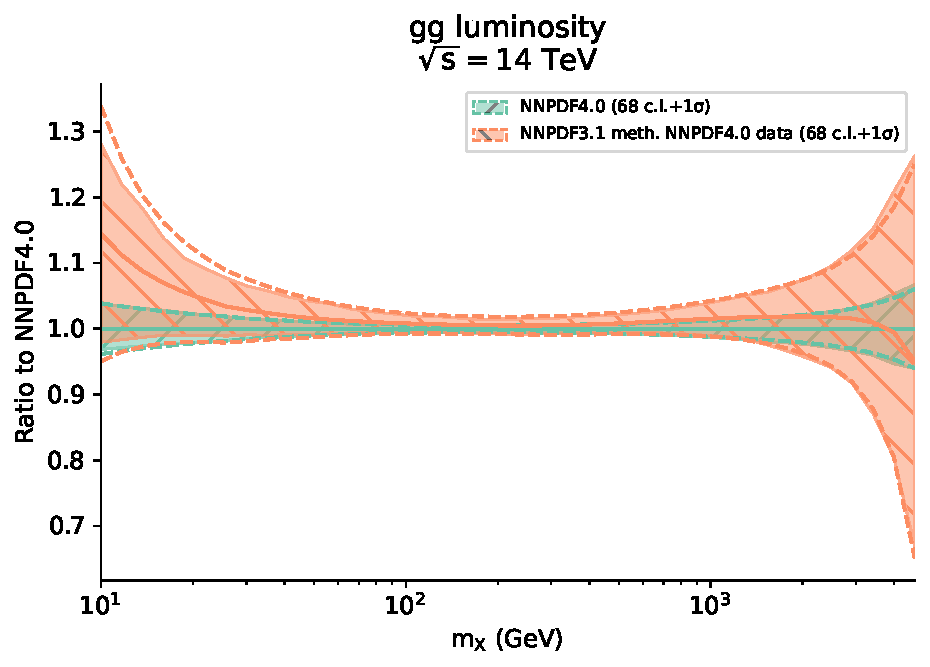
\includegraphics[width=0.45\textwidth]{lumi1d_gg_NNPDF31meth_NNPDF40data}
	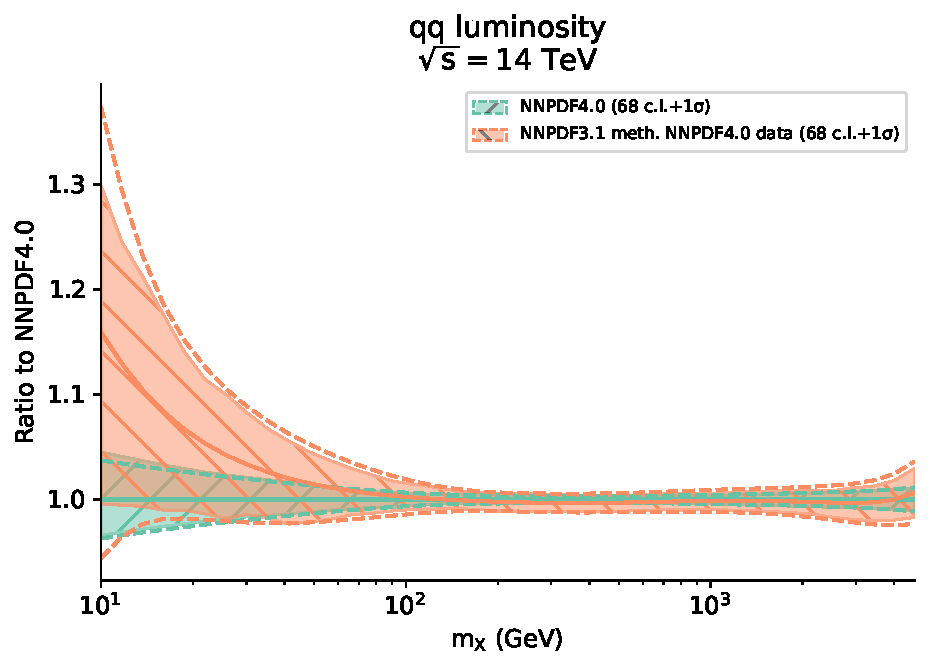
\includegraphics[width=0.45\textwidth]{lumi1d_qq_NNPDF31meth_NNPDF40data}
	\begin{columns}
	    \column{0.45\linewidth}
			\begin{itemize}
	    	        \item Significant reduction of PDF uncertainties
		        \item Good agreement between the central values
		    \end{itemize}
        \column{0.5\linewidth}
            \begin{block}{}
                \fontsize{7}{6}\selectfont
                PDF uncertainties are validated using closure tests and future tests\\
                Validation tests successful for both NNPDF4.0 and NNPDF3.1 
            \end{block}
    \end{columns}
\end{frame}



\begin{frame}[t]{Implications for phenomenology}
    \begin{center}
        Reduced luminosity uncertainties $\rightarrow$ Reduced uncertainty at the level of observables\\
        \vspace*{-0.5em}
        \begin{columns}
	        \begin{column}{0.48\textwidth}
	            \begin{center}
	                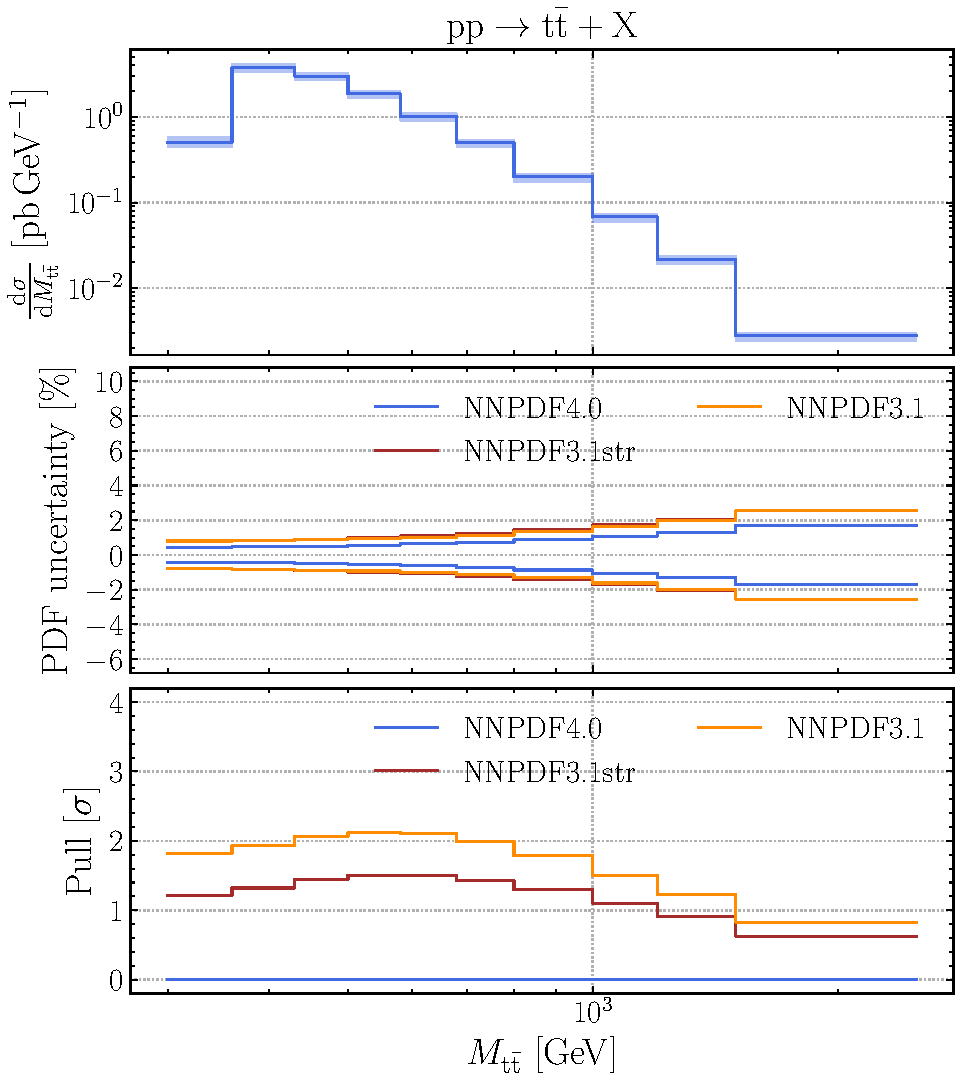
\includegraphics[width=0.78\textwidth]{NNPDF_TTB_14TEV_40_PHENO-internal} 
	            \end{center}
	        \end{column}
	        \begin{column}{0.48\textwidth}
	            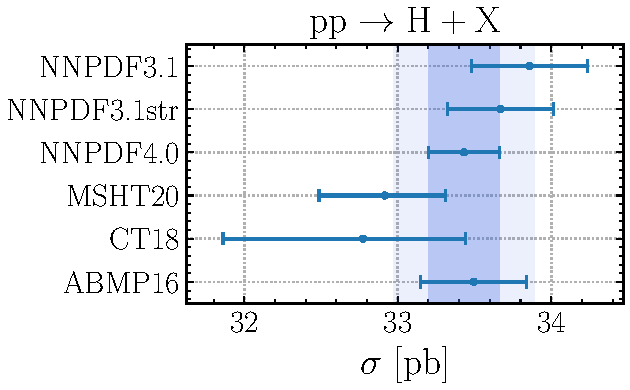
\includegraphics[width=0.7\textwidth]{NNPDF_H_14TEV_40_PHENO-integrated}\\
        	        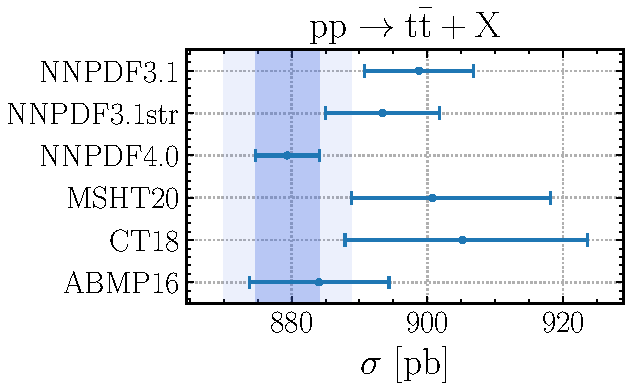
\includegraphics[width=0.7\textwidth]{NNPDF_TTB_14TEV_40_PHENO-integrated}
	        \end{column}
        \end{columns}
    \end{center}
\end{frame}

%\begin{frame}{Implications for phenomenology}
%    \begin{center}
%        Reduced luminosity uncertainties $\rightarrow$ Reduced uncertainty at the observable level
%        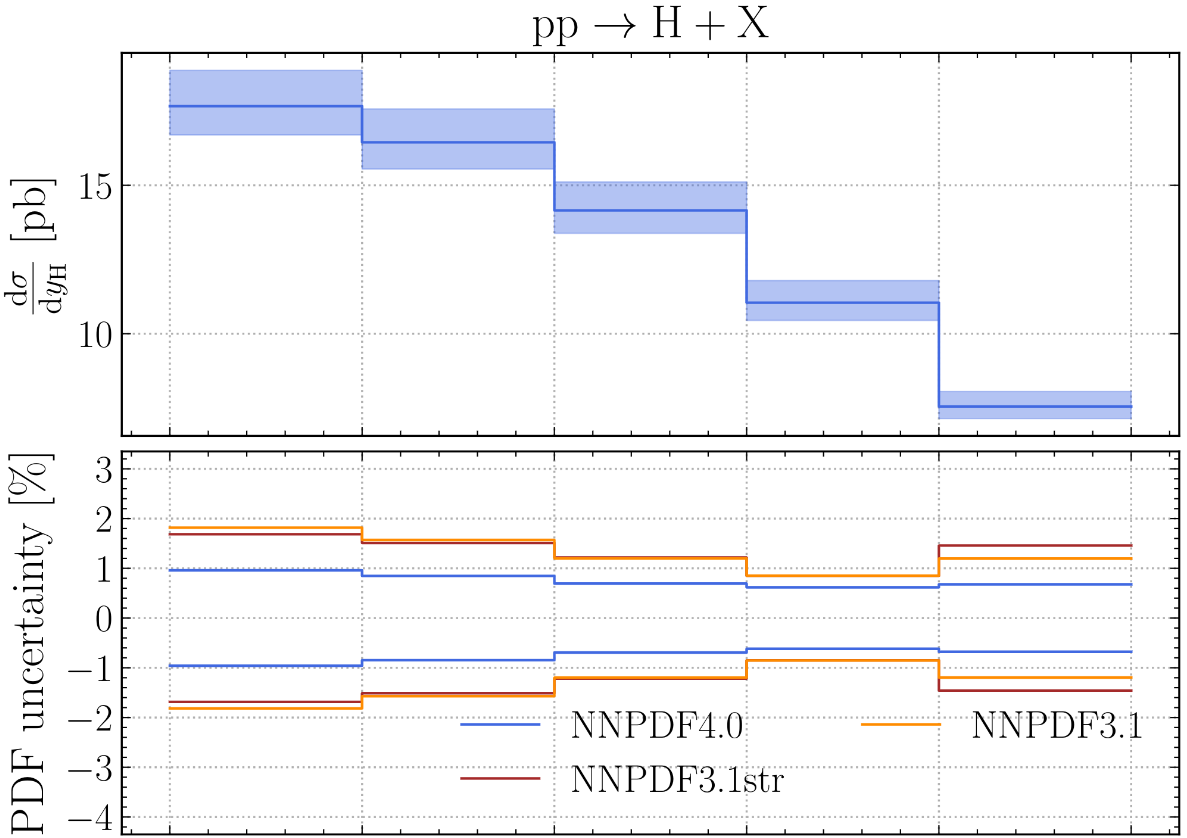
\includegraphics[width=0.55\textwidth]{pheno_h}
%    \end{center}
%\end{frame}




\section*{Conclusions}



\begin{frame}[t]{Summary}
    \begin{itemize}
        \item Added $\mathcal{O}(400)$ new data points from many new processes
        \item Improved methodology with Stochastic Gradient Descent and hyperoptimization
        \item Validation of PDF uncertainties using closure test, future test and parametrization basis independence
        \item[$\Rightarrow$] NNPDF4.0 achieves a high precision over a broad kinematic range
    \end{itemize}
    \vspace*{2em}
    \begin{block}{}
        \centering
        {\bf NNPDF code} will be made {\bf publicly available} along with user-friendly documentation
    \end{block}
    \vspace*{2em}
    \only<2>{
    \begin{center}
        {\vspace*{2em} \Large \textbf{Thank you!}}
    \end{center}
    }
\end{frame}



\begin{frame}{Determination of the photon PDF}
  \begin{columns}[T]
    \begin{column}{0.59\textwidth}
      Initially the photon PDF has been determined in different ways:
      \begin{itemize}
        \item physical model: sensitive to underlying model
        \item fitting: data does not provide strong constraints
      \end{itemize}

      \vspace*{0.5em}
      However with the LUXqed approach it can be computed perturbatively \\
      based on the observation that the heavy-lepton production cross-section can be written in two ways:
      \begin{itemize}
        \item in terms of structure functions $F_2$, $F_L$
        \item in terms of PDFs (including the photon)
      \end{itemize}

      \vspace*{0.5em}
      luxQED result {\color{gray}\small[Manohar, Nason, Salam, Zanderighi: 1607.04266, 1708.01256]}:
      \vspace*{-0.8em}
      \begin{equation*}
        \begin{split}
          & x \gamma(x, \mu^2)
          =
          \frac{2}{\alpha (\mu^2)} \int\limits_x^1 \frac{dz}{z}
          \Biggl\{ \int_{m_p^2x^2 \over 1-z}^{\mu^2 \over 1-z} \frac{dQ^2}{Q^2}
          \alpha^2(Q^2) \Biggl[ -z^2 F_L(x/z, Q^2) \\
          & + \left( z P_{\gamma q}(z) + \frac{2 x^2 m_p^2}{Q^2} \right)
          F_2(x/z, Q^2)\Biggr] - \alpha^2(\mu^2) z^2 F_2(x/z, \mu^2)\Biggr\}
        \end{split}
      \end{equation*}
    \end{column}

    \begin{column}{0.39\textwidth}
      \vspace*{-2.5em}
      \begin{figure}
        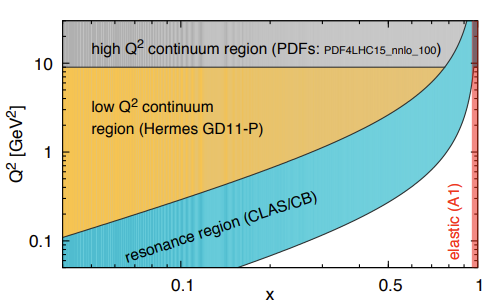
\includegraphics[width=0.89\textwidth]{figures/dataluxqed.png}
        \caption*{Input to construct $F_2$ and $F_L$}
        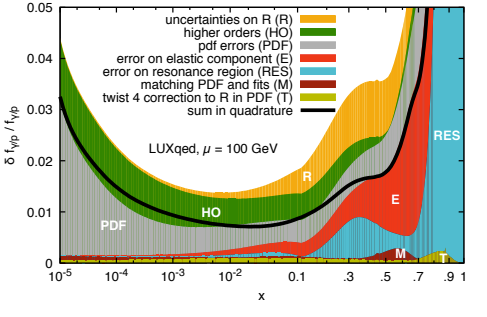
\includegraphics[width=0.89\textwidth]{figures/luxQED_uncs.png}
        \caption*{Sources of uncertainty}
      \end{figure}
    \end{column}
  \end{columns}
\end{frame}


\begin{frame}{LUXqed PDF determinations}
  LUXqed has been used in all of the most recent QED PDFs:
  \begin{itemize}
      \item LUXqed\_plus\_PDF4LHC15 {\color{gray}\small [1607.04266]}
      \item LUXqed17\_plus\_PDF4LHC15 {\color{gray}\small [1708.01256]}
      \item MMHT2015qed {\color{gray}\small [1907.02750]}
      \item NNPDF3.1luxQED {\color{gray}\small [1712.07053]}
      \item CT18lux and CT18qed {\color{gray}\small [2106.10299]}
      \item MSHT20QED {\color{gray}\small [2111.05357]}
      \item MSHT20qed\_an3lo {\color{gray}\small [2312.07665]}
      \item NNPDF4.0QED {\color{gray}\small [2401.08749 ]}
  \end{itemize}
\end{frame}

% \begin{frame}{Results: photon PDF and luminosity}
%   \begin{center}
%     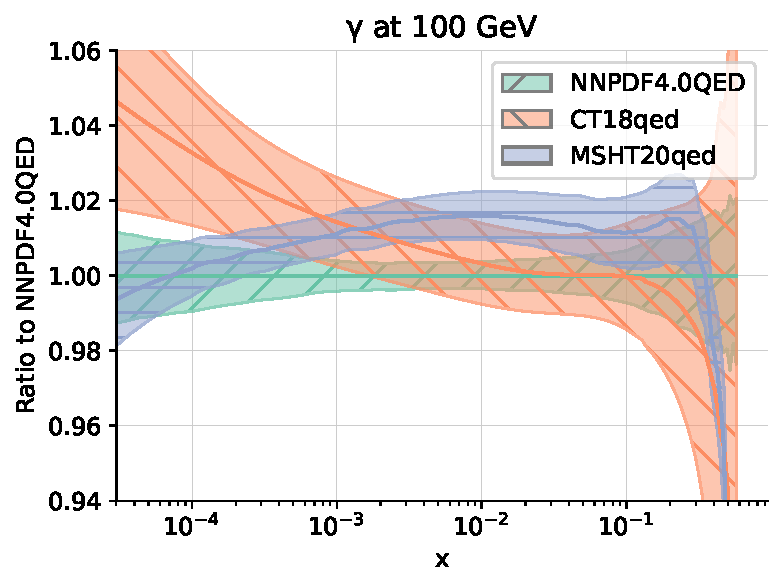
\includegraphics[width=0.3\textwidth]{figures/photon_comparison.pdf}
%     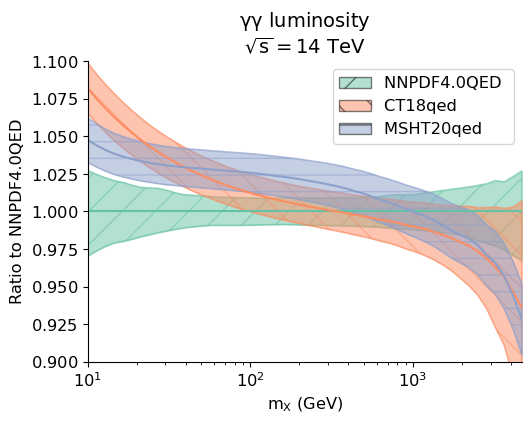
\includegraphics[width=0.3\textwidth]{figures/pp_lumi_comparison.png}
%     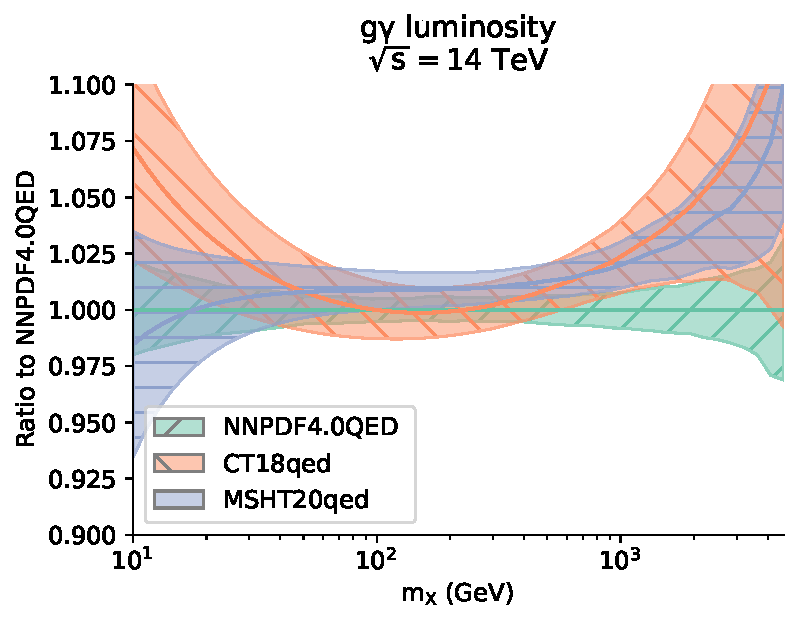
\includegraphics[width=0.3\textwidth]{figures/gp_lumi_comparison.pdf}
%   \end{center}
%   \begin{itemize}
%     \item Because all groups use the luxQED formalism, the photon PDFs agree at percent level
%     \item Luminosity generally in agreement, but differ at very small and very large invariant mass
%   \end{itemize}
% \end{frame}


% ============================================================================


\begin{frame}{Incomplete higher order uncertainties covmat}
  \begin{itemize}
    \item We construct an IHOU matrix following a similar approach by varying the subleading functions
    \item IHOU are independent of MHOU so the uncertainties are added in quadrature
    $$C = C_\mathrm{exp}+C_\mathrm{MHOU}+C_\mathrm{IHOU}$$
  \end{itemize}

  \begin{columns}
    \begin{column}{0.49\textwidth}
      \begin{figure}[!t]
        \centering
        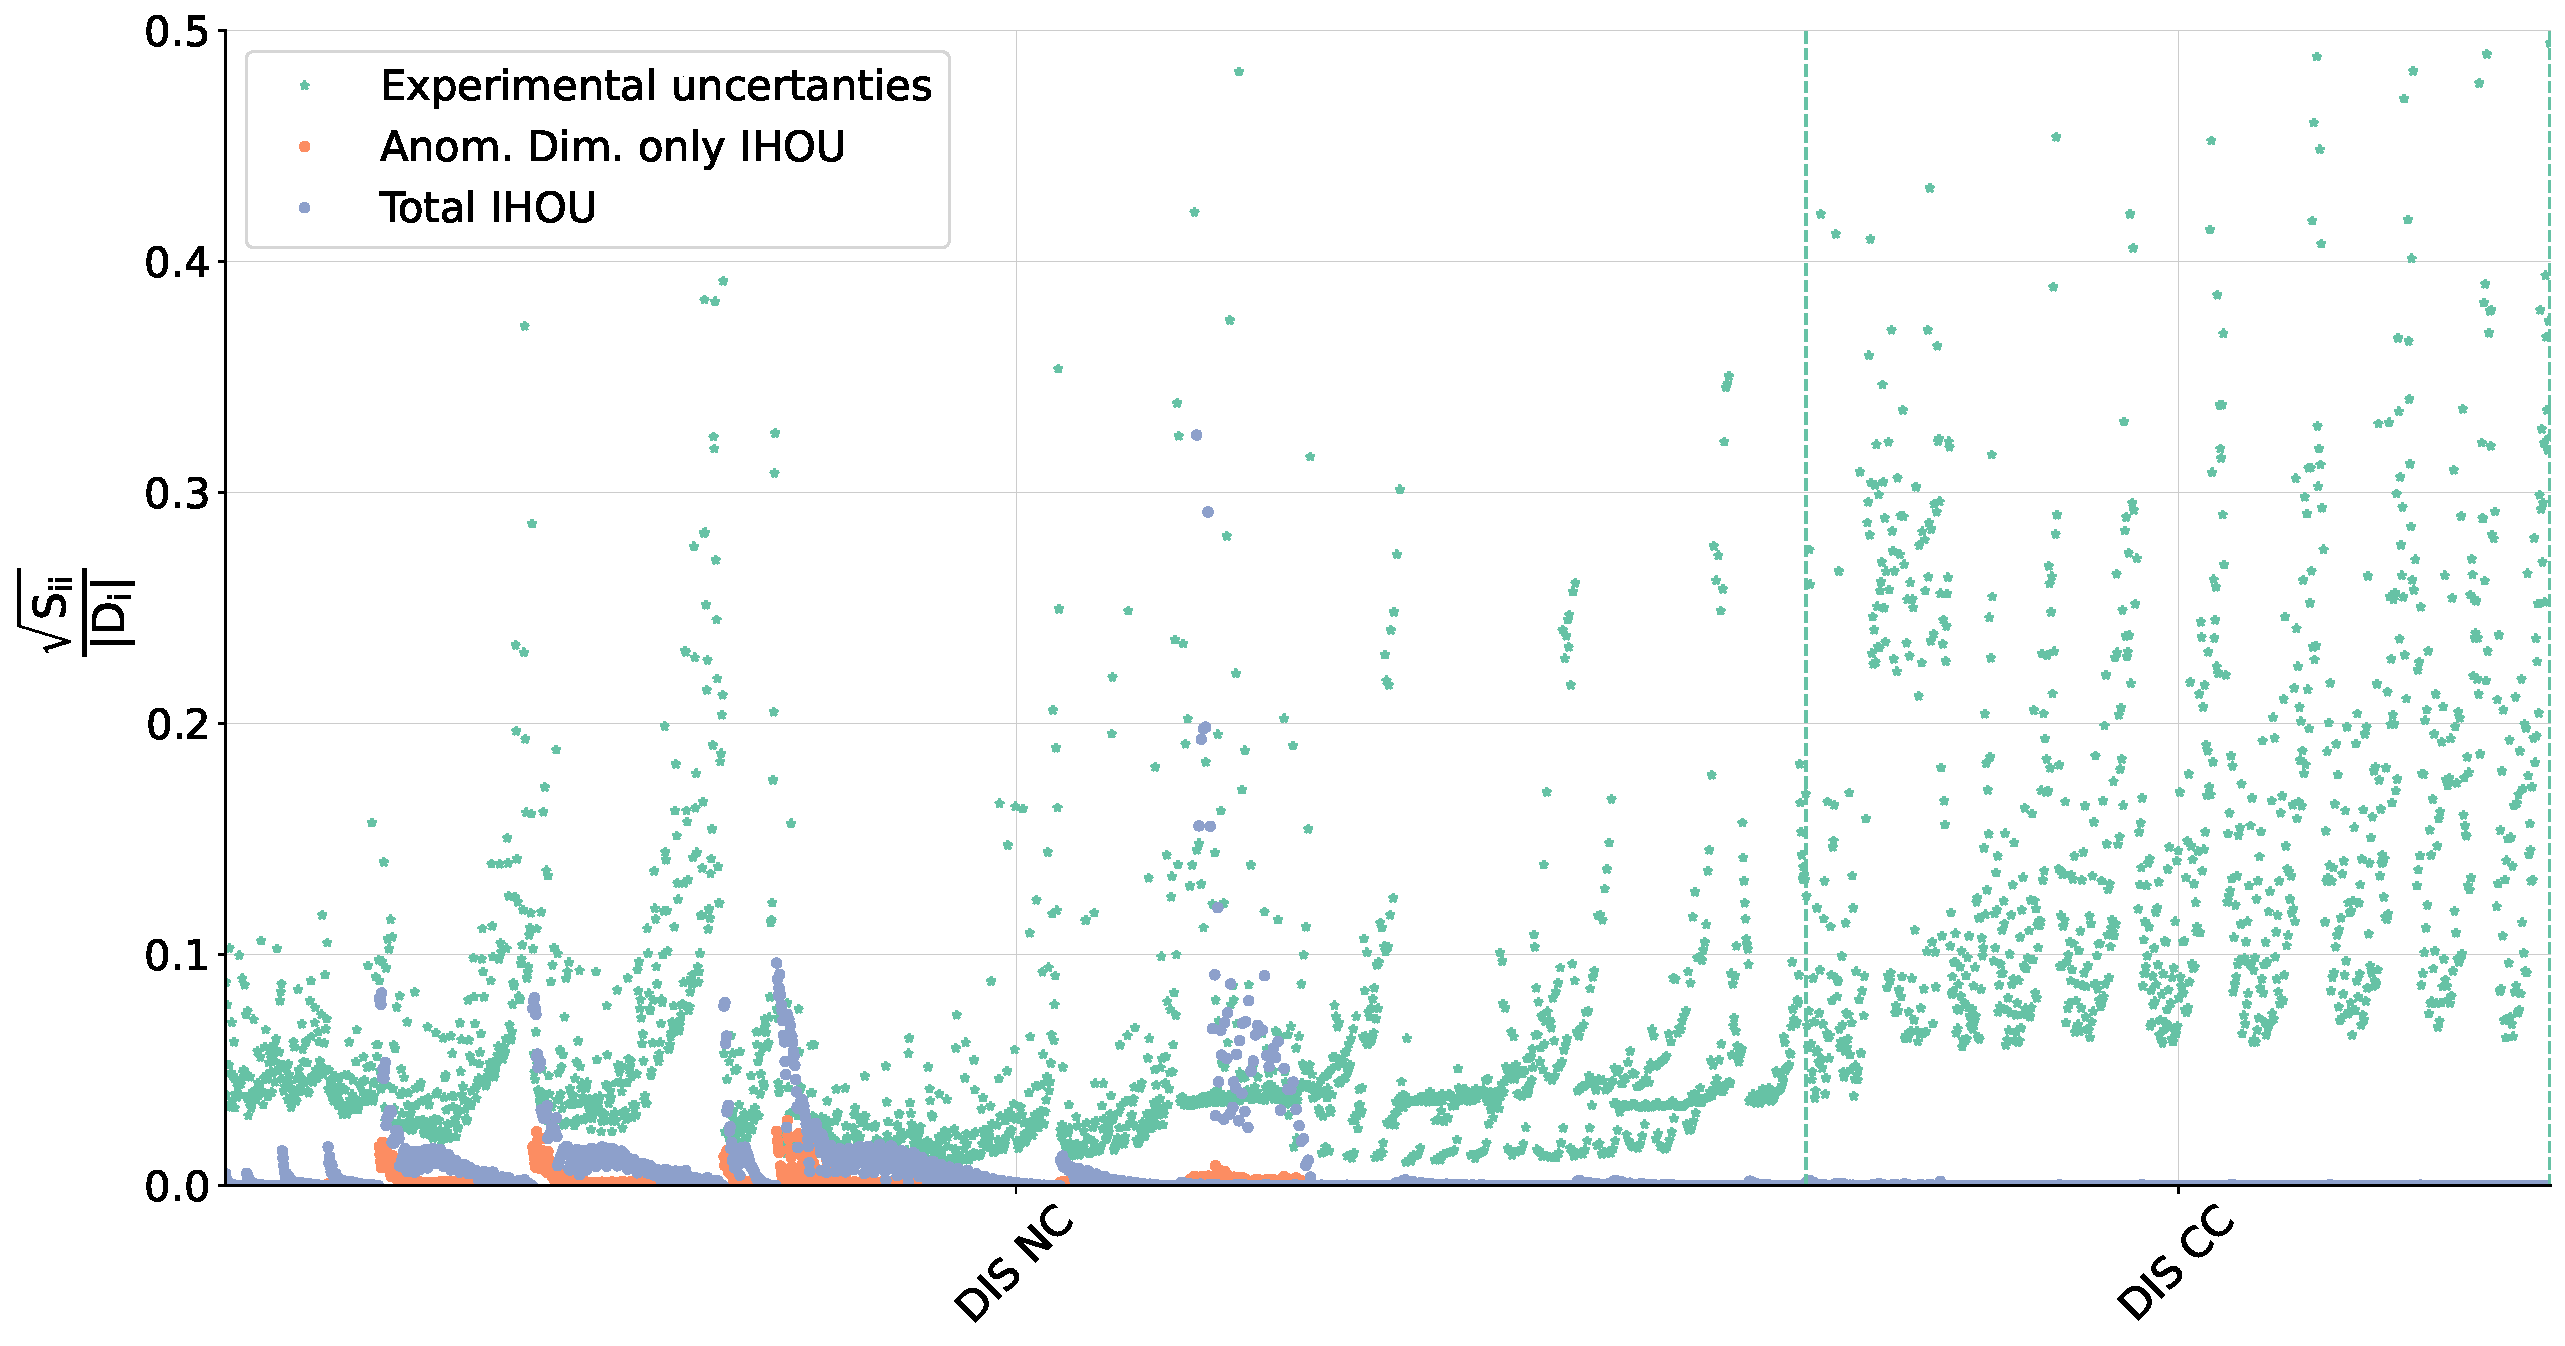
\includegraphics[width=.9\textwidth]{figures/diag_cov_dis_ihou.pdf}
        \caption*{IHOU have a large effect on small-$x$, low-$Q$ DIS data
        }
      \end{figure}
    \end{column}
    \begin{column}{0.49\textwidth}
      \begin{figure}[!t]
        \centering
        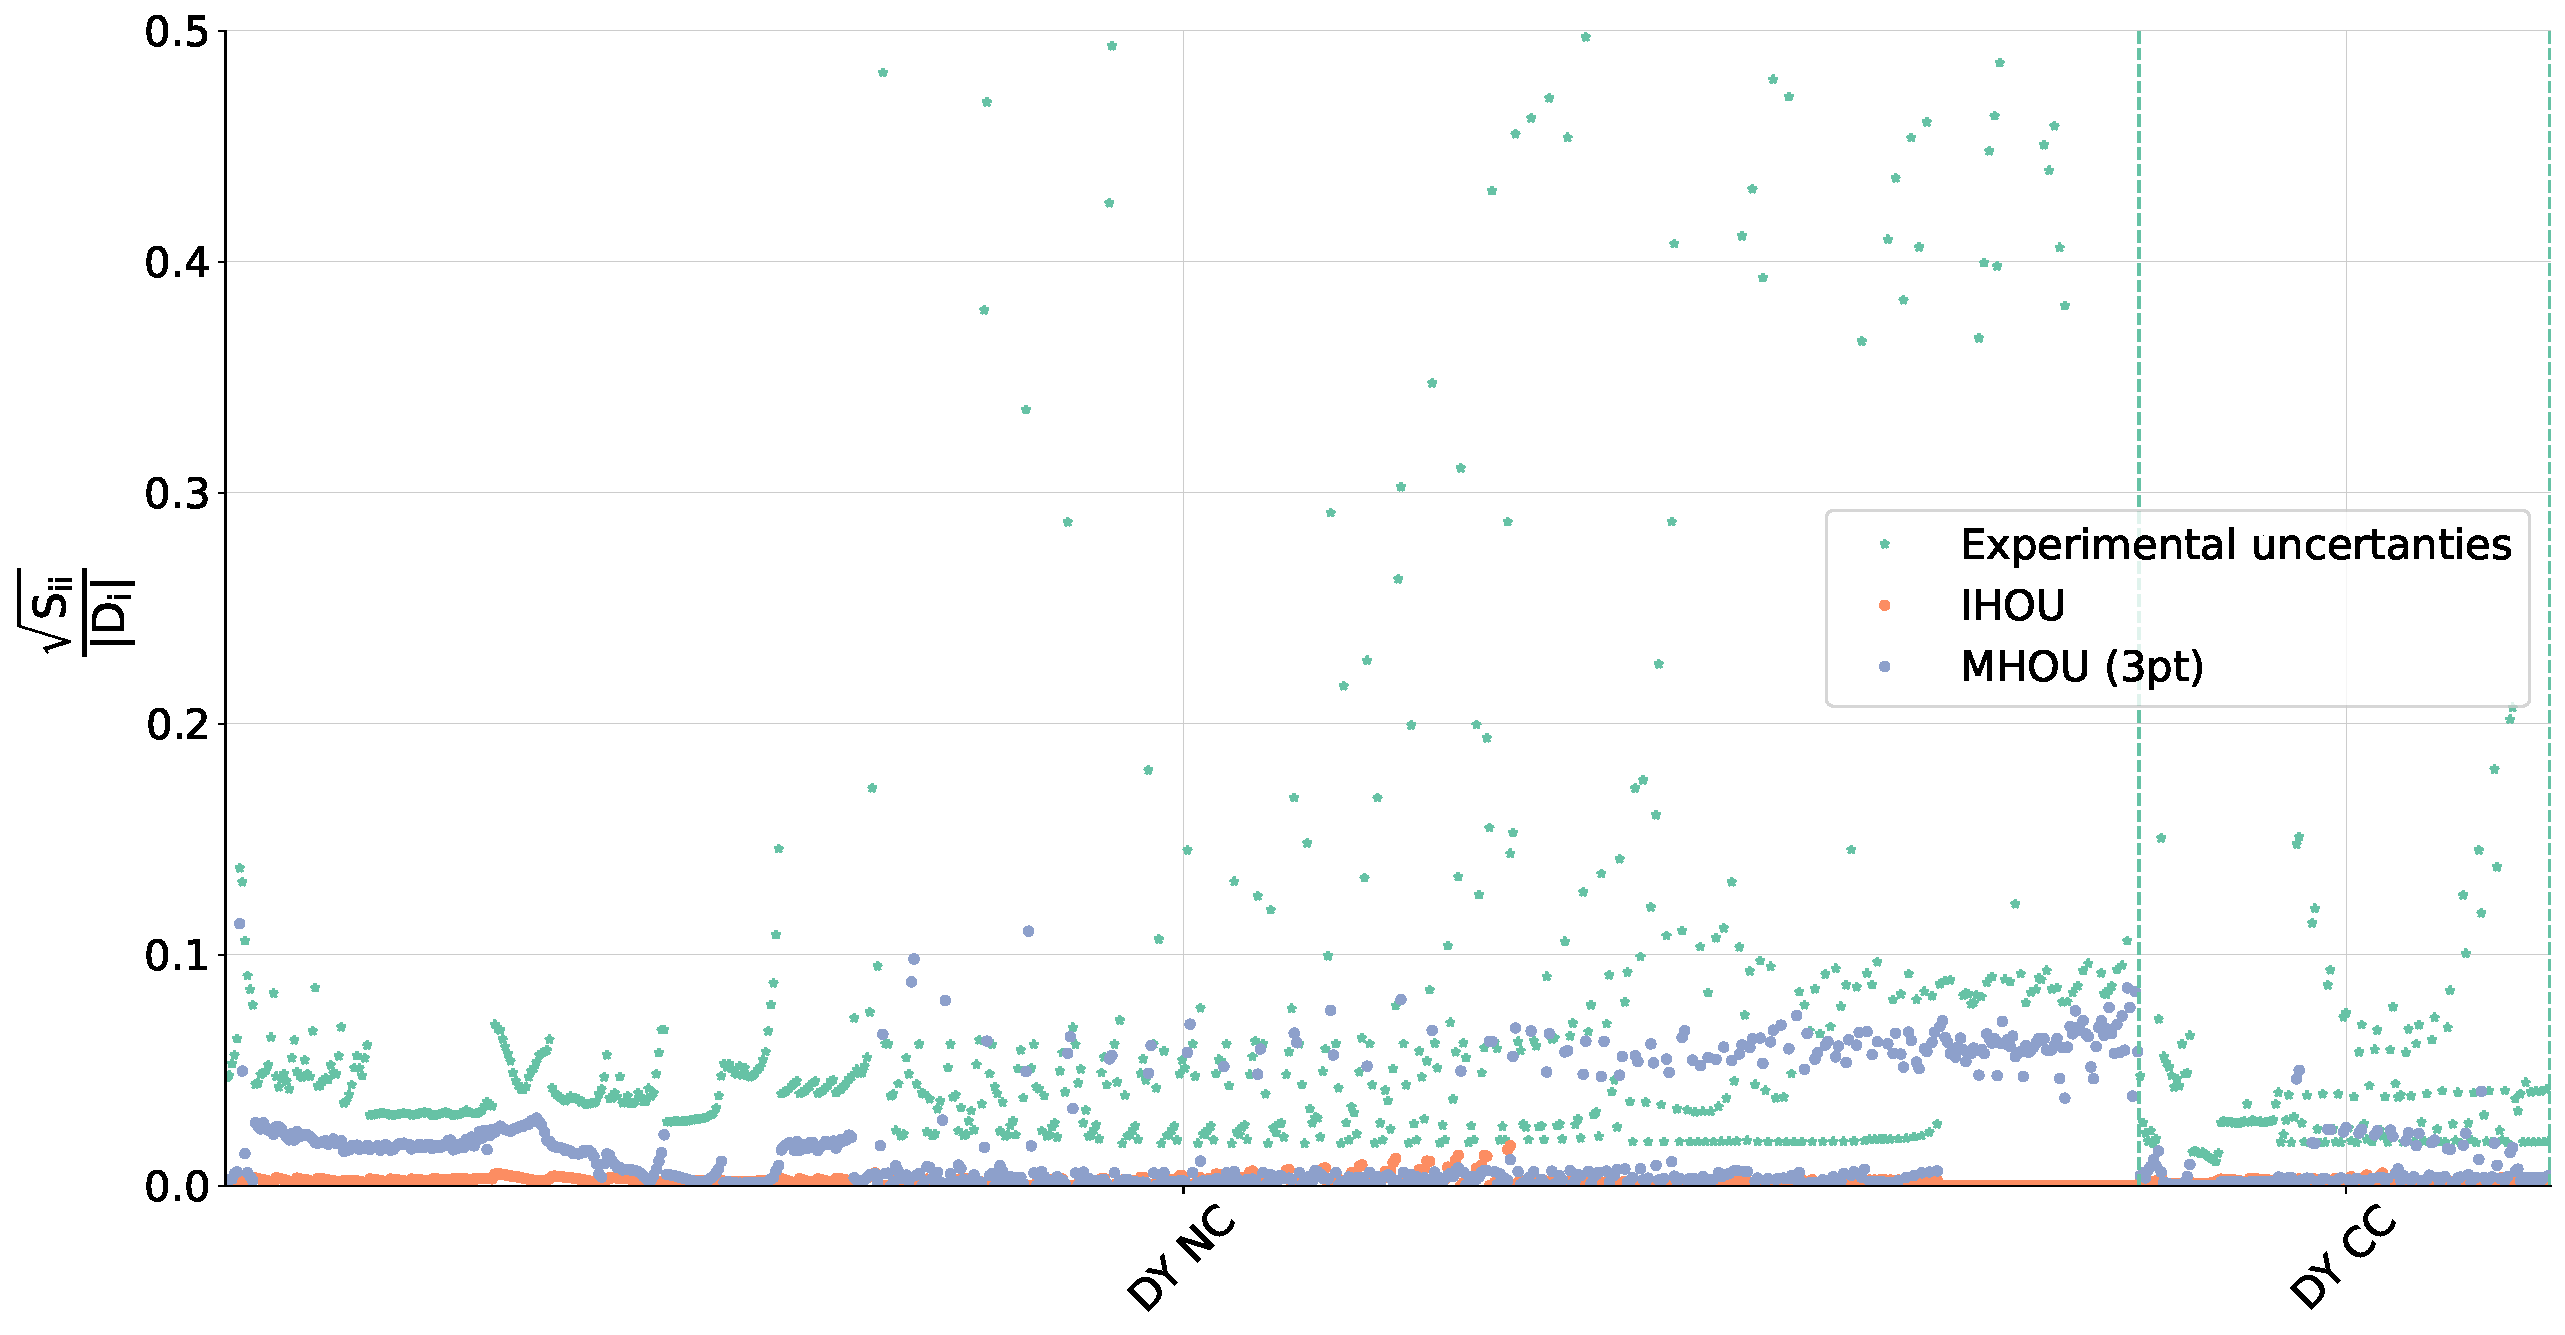
\includegraphics[width=.9\textwidth]{figures/diag_cov_dy_ihou_3pt_mhou.pdf}
        \caption*{NNLO MHOU included where N3LO not available \\
          MHOU can similar magnitude as the experimental uncertainty
        }
      \end{figure}
    \end{column}
  \end{columns}


\end{frame}

% \begin{frame}{Magnitude of theory uncertainties}
% % show that for certain processes th unc is of same size as exp unc.
% \end{frame}

% ============================================================================

\begin{frame}{Impact of MHOUs at N3LO}
  \begin{figure}[!t]
    \centering
    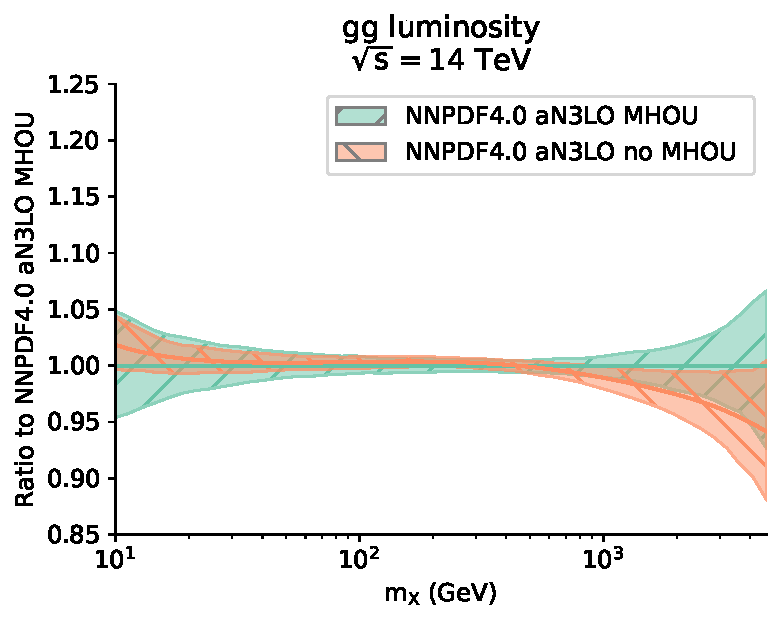
\includegraphics[width=0.45\textwidth]{figures/gg_plot_lumi1d.pdf}
    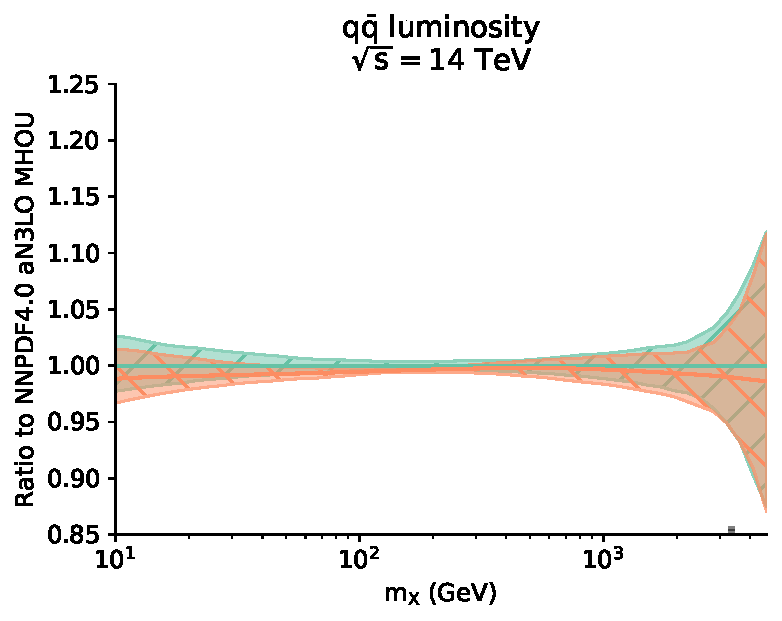
\includegraphics[width=0.45\textwidth]{figures/qqbar_plot_lumi1d.pdf}
  \end{figure}
  \begin{itemize}
    \item Non-negligible impact of MHOUs even at N3LO
    \item[$\Rightarrow$] reason to include exact N3LO calculations for hadronic processes
  \end{itemize}
\end{frame}


% \begin{frame}{Comparison to MSHT20}
%   \begin{figure}[!t]
%     \centering
%     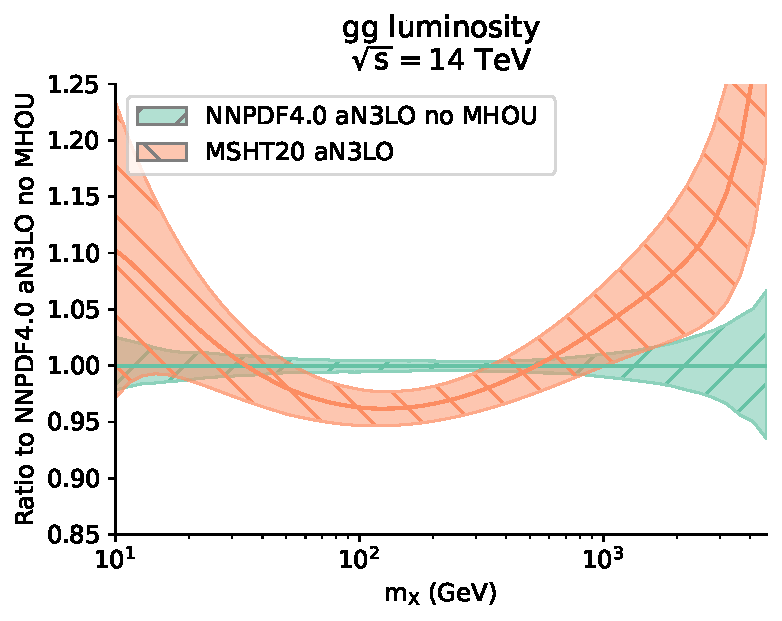
\includegraphics[width=0.45\textwidth]{figures/gg_plot_lumi1d_msht20.pdf}
%     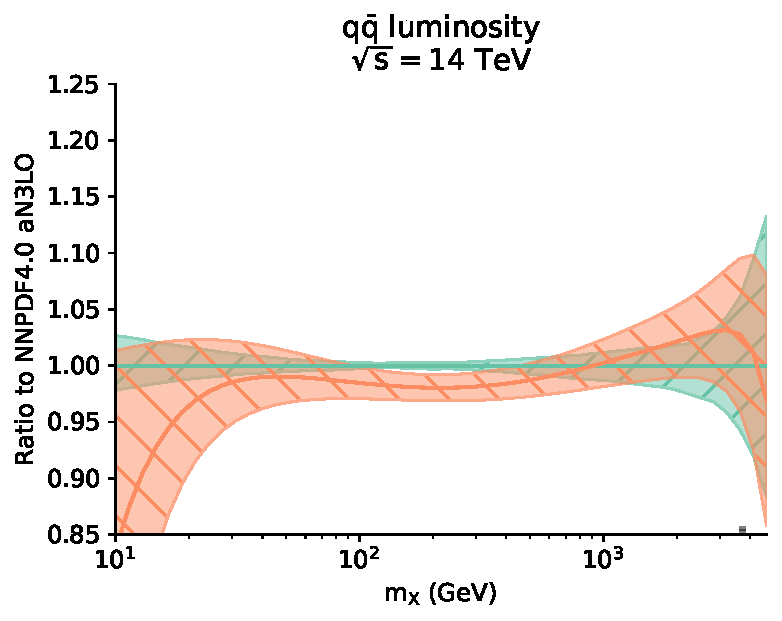
\includegraphics[width=0.45\textwidth]{figures/qqbar_plot_lumi1d_msht20.pdf}
%   \end{figure}
%   \begin{itemize}
%     \item Good agreement with MSHT20 for the quark luminosities
%     \item Also for gluon luminosities, except around the Higgs mass and high-mass
%     \item Similar data but different methodology (including splitting function parametrization)
%   \end{itemize}
% \end{frame}









\end{document}
